% !TEX root = ../McCoy-Dissertation.tex
\Appendix{Scalar Treatment of Gratings}\label{ap:grating_basics}
%%%%%%%%%%%%%%%%%%%%%e%%%%%%%%%%%%%%%%%%%%--------------------------------------------------
As motivated in \cref{sec:grating_tech_dev}, diffraction gratings are the instrument of choice for sensitive, high-resolution spectroscopy in the soft x-ray spectrum, particularly for the photon-energy range $\SI{250}{\electronvolt} \lessapprox \mathcal{E}_{\gamma} \lessapprox \SI{1}{\kilo\electronvolt}$, where energy-dispersive detectors intended for higher-energy x-rays face limitations in terms of spectral resolving power, $\mathscr{R}$. 
While x-rays are often associated with their particle-like behavior [\emph{cf.\@} \cref{ap:x-ray_intro}], like all types of waves they experience the phenomenon of diffraction as they bend around obstacles, spread outward from narrow openings or otherwise superpose to produce interference patterns.\footnote{An everyday example of this phenomenon is waves on the surface of a shallow pond, which undergo diffraction as they pass through a narrow opening created by protruding rocks, or when multiple waves from splashes overlap to produce interference fringes.} 
Fundamentally, this behavior arises because according to the \emph{Huygens-Fresnel principle}, any given wavefront can be understood as being composed of a set of point sources that emanate secondary spherical waves \cite{Born80}. 
This implies that when a wave encounters an aperture, the scenario is equivalent to there being a new distribution of point sources that interfere with one another as they propagate, producing diffraction patterns. 
As these secondary waves move forward, they interfere with one another to form the diffracted wavefront. 
In the case of multiple obstacles or openings, an additional diffraction pattern is produced as the wavefronts from each aperture overlap and produce interference fringes. 
For a large number of evenly-spaced apertures, the system behaves like a diffraction grating, where an ordered interference pattern is produced in the far field that depends on the spatial periodicity, the wavelength and the angle of incidence \cite{Loewen97}. 

Considering wave mechanics alone, a diffraction grating for soft x-rays can be realized as a periodic structure with a very fine pitch to accommodate the wavelength of radiation $\SI{5}{\nm} \gtrapprox \lambda = h c_0 / \mathcal{E}_{\gamma} \gtrapprox \SI{1.25}{\nm}$. 
However, when the interaction of radiation with matter is taken into account [\emph{cf.\@} \cref{app:x-ray_materials}], soft x-rays and other short-$\lambda$ radiation are found to reflect appreciably only at grazing incidence angles in the regime of \emph{total external reflection}. 
This restriction introduces practical challenges and drives the consideration of alternative grating geometries that produce conical diffraction patterns from oblique angles of incidence. 
To introduce these concepts and ultimately motivate the specifics of what goes into the design of efficient reflection gratings for soft x-ray spectroscopy, this appendix outlines basic physics of diffraction gratings according to scalar theories of diffraction, which, by construction, ignore effects related to the polarization of electromagnetic radiation and the atomic structure of materials. 
In this case, scalar waves are imagined to diffract from idealized structures that scale equally with any wavelength so that according to the Huygens-Fresnel principle, a grating can be described as a continuous surface of point sources with periodic variations in amplitude, phase or both. 
While the electromagnetic vector treatment of gratings outlined in \cref{sec:integral_method} is needed to describe these phenomena most accurately, scalar theories of diffraction can be used to describe roughly the behavior of diffraction gratings, including the effect that groove shape has on the dispersed radiation. 

\section{Wave Interference From an Array of Slits}\label{sec:slit_array}
%%%%%%%%%%%%%%%%%%%%%%%%%%%%%%%%%%%%%%%%%--------------------------------------------------
As a first step toward describing diffraction gratings, a generic, scalar plane wave of wavelength $\lambda$ is imagined to be incident on a barrier with two narrow slits\footnote{The lengths of these slits are taken to be formally infinite so that this scenario can be treated two-dimensionally. In other words, each aperture is considered to be sufficiently long such that diffraction from edge effects along this direction can be neglected.} separated by a distance $d$, each with a width $W \ll \lambda$ so that both can be thought of as the source of a true circular wave according to the Huygens-Fresnel principle.
This is illustrated in \cref{fig:double_slit_experiment}, where the barrier lays in the plane defined by the $x$-axis and the direction pointing out of the page.
\begin{figure}
 \centering
 \includegraphics[scale=1.07]{Appendix-D/Figures/path_length5.mps}
 \caption{Near-field interference from two very small slits}\label{fig:double_slit_experiment}
 \end{figure}
Initially, it is assumed that the incident wave vector, $\mathbold{k}$ (with $\abs{\mathbold{k}} \equiv k = 2 \pi / \lambda$) is oriented perpendicular to this barrier so that the incident wave propagates in the $y$-direction, $\mathbold{\hat{y}}$, with a scalar field satisfying \cref{eq:scalar_wave_general} of the form 
\begin{equation}
 u(y,t) \propto \mathrm{e}^{i \left( k y - \omega t \right)} ,
 \end{equation}
where $\omega = 2 \pi c / \lambda$ is the frequency of the wave and $c$ is the speed of the wave. 
Meanwhile, each slit emanates circular waves that can be expressed in polar coordinates, $\mathbold{s} \equiv (s, \vartheta)$, as 
\begin{equation}\label{eq:circular_wave}
 u(s,t) \propto \frac{1}{\sqrt{s}} \, \mathrm{e}^{i \left( k s - \omega t \right)} ,
 \end{equation}
where $s \equiv \sqrt{x^2 + y^2}$ is a 2D radial distance and $\vartheta \equiv - \arccos \left( x /s \right)$ for $y \geq 0$. 
As indicated in \cref{fig:double_slit_experiment}, the incident planar wave gives rise to two point sources, $S_1$ and $S_2$, at the location of each slit: $(x,y) = (\pm d/2,0)$ relative to the $x-y$ origin, $O$. 
These two sources separately define scalar waves $u_1 (s_1,t)$ and $u_2 (s_2,t)$ of the form given in \cref{eq:circular_wave}, where $s_1$ and $s_2$ are the radial distances from each slit. 

The interference pattern caused by the placement of these sources is determined by probing the intensity of the combined scalar wave $u ( \mathbold{s} , t ) = u_1 ( \mathbold{s} , t ) + u_2 ( \mathbold{s} , t )$ at some fixed point, $P_0$, away from the barrier. 
With the magnitude of \emph{Poynting's vector}, $\mathbold{S}$, being proportional to $\norm{u}^2$, the double-slit \emph{interference function} is taken to be $I_2 \propto \norm{u}^2$, where the maximum of the function is normalized to unity. 
Shown in \cref{fig:double_slit_experiment}, this arbitrary point where wave intensity\footnote{As described in \cref{sec:amplitude_phase}, the wave intensity, $\mathcal{I}$, that passes through a plane parallel to the barrier depends on $\vartheta$ such that $\mathcal{I} \equiv \mathbold{S} \cdot \mathbold{\hat{y}} \propto \norm{u}^2 \cos \left( \vartheta \right)$.} is imagined to measured is located a distance $L$ from the barrier so that radial distance from $O$ to $P_0$ is $r_0 = L \sec (\vartheta)$. 
Because the incident wavefronts are assumed to be oriented parallel to the barrier, sources $S_1$ and $S_2$ generate waves with identical amplitude and phase. 
However, by the time their wavefronts reach $P_0$, there will generally be differences in amplitude and phase due to the fact that there is a \emph{path-length difference}, $\Delta s \equiv s_2 - s_1 \equiv \overline{S_2 Q}$, where $s_1 \equiv \overline{S_1 P_0}$ and $s_2 \equiv \overline{S_2 P_0}$ in \cref{fig:double_slit_experiment}. 
These path lengths $s_1$ and $s_2$ can be determined using the \emph{law of cosines}: 
\begin{align}
 \begin{split}
 s_1^2 &= \left( \frac{d}{2} \right)^2 + r_0^2 - r_0 \, d \cos \left(\frac{\pi}{2} - \vartheta \right) = \left( \frac{d}{2} \right)^2 + L^2 \sec^2 \left( \vartheta \right) - L \, d \tan \left( \vartheta \right) \\
 s_2^2 &= \left( \frac{d}{2} \right)^2 + r_0^2 - r_0 \, d \cos \left(\frac{\pi}{2} + \vartheta \right) = \left( \frac{d}{2} \right)^2 + L^2 \sec^2 \left( \vartheta \right) + L \, d \tan \left( \vartheta \right) . \label{eq:path_length_exact}
 \end{split}
 \end{align} 
In terms of \cref{fig:double_slit_experiment}, sources $S_1$ and $S_2$ have radial distances $s_1$ and $s_2$ to $P_0$ while the amplitudes of the $S_1$ and $S_2$ wavefronts are defined to be $\mathcal{A}_1$ and $\mathcal{A}_2$, respectively. 
Especially for small $L$, the difference between these amplitudes depends on $s_1$ and $s_2$ separately, instead of $\Delta s$. 
On the other hand, the $S_2$ wavefront is shifted by a phase $\Phi = - k \Delta s$ relative to the $S_1$ wavefront. 
Using this notation, the $S_1$ scalar field at $P_0$ is $u_1 (t) \equiv \mathcal{A}_1 \mathrm{e}^{- i \omega t}$ and the $S_2$ scalar field at $P_0$ is $u_2 (t) = \mathcal{A}_2 \mathrm{e}^{i (\Phi -  \omega t)}$ with the overall wave at this point being described by 
\begin{equation}\label{eq:scalar_field_double_slit}
 u (t) = u_1 (t) + u_2 (t) = \mathrm{e}^{- i \omega t} \left( \mathcal{A}_1 + \mathcal{A}_2 \mathrm{e}^{i \Phi} \right) \quad \text{for 2 slits} .
 \end{equation}

As a next step toward describing a diffraction grating, the \emph{far-field approximation} is invoked such that the distance to $P_0$ is taken to be very large compared to the spacing between the slits so that $L \gg d$ and rays $\overrightarrow{S_1 P_0}$ and $\overrightarrow{S_2 P_0}$ are approximately parallel to each other. 
\begin{figure}
\centering
\includegraphics[scale=1.07]{Appendix-D/Figures/path_length4.mps}
\caption{Far-field interference from two very small slits}\label{fig:double_slit_experiment_approx}
\end{figure}
This scenario is illustrated in \cref{fig:double_slit_experiment_approx}, where $P_0$ is effectively at an infinite distance from the barrier.  
In this case, $r_0 \gg \Delta s$ and the diffracted wavefronts are roughly planar with $\mathcal{A}_1 \approx \mathcal{A}_2 \equiv \mathcal{A}_0$, where $\mathcal{A}_0$ is the amplitude measured at $P_0$. 
Using the approximation $s_2 + s_1 \approx 2 r_0$, the difference of the two terms in \cref{eq:path_length_exact} becomes 
\begin{equation}
 s_2^2 - s_1^2 = 2 L \, d \tan \left( \vartheta \right) = \left( s_2 + s_1 \right) \left( s_2 - s_1 \right) \approx 2 L \sec \left( \vartheta \right) \Delta s 
 \end{equation}
and, therefore, the path-length difference in the far field is $\Delta s = d \sin (\vartheta)$ assuming that the incident wave is normally incident on the barrier. 
The phase shift is $\Phi = - k \Delta s$ with the double-slit interference function given by
\begin{equation}\label{eq:double-slit_intensity}
 I_2 \left( \Phi \right) \propto \norm{u ( t )}^2 = 2 \mathcal{A}_0^2 \left[ 1 + \cos \left( \Phi \right) \right] \quad \text{for 2 slits,}
 \end{equation}
where $u (t)$ follows from \cref{eq:scalar_field_double_slit} using $\mathcal{A}_1 = \mathcal{A}_2 = \mathcal{A}_0$. 
Maxima of this function correspond to $\Phi = 2 n \pi$ or, equivalently, $\Delta s = - n \lambda$ with $n = 0, \pm 1, \pm 2, \pm 3 \dotsc$  
Physically, these maxima represent constructive interference fringes with angular locations given by 
\begin{equation}\label{eq:fringes}
 \sin \left( \vartheta_{\text{max}} \right) = - \frac{n \lambda}{d} \quad \text{for } n = 0, \pm 1, \pm 2, \pm 3 \dotsc 
 \end{equation}
provided that $-1 < n \lambda / d < 1$. 
\begin{figure}
\centering
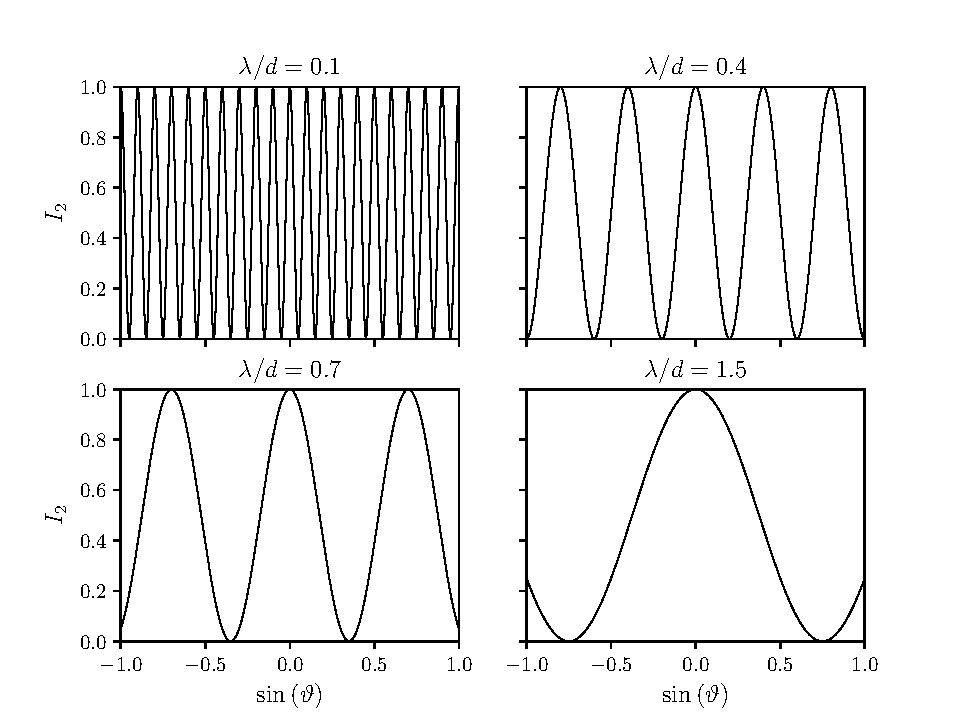
\includegraphics[scale=0.99]{Appendix-D/Figures/double_slit_plots.pdf}
\caption[Normalized interference function for two point sources for various wavelengths]{Normalized interference function for two point sources as a function of $\sin (\vartheta)$ for various $\lambda / d$ ratios.}\label{fig:double_slit_plot}
\end{figure} 
The sinusoidal dependence of the far-field double-slit interference pattern on $k d$, and hence the ratio $\lambda / d$, is demonstrated in \cref{fig:double_slit_plot}. 

The double-slit scenario outlined above can be generalized to $N$ equally-spaced slits, each an identical source $S_m$ (for $m = 1, 2, \dotsc , N$). 
In this case, $P_0$ is considered to be a distance $L \gg (N - 1) d$ away from the barrier so that far-field approximations are valid. 
At $P_0$, the amplitude associated with each slit is virtually the same in this approximation so that the scalar field at this point due to the $m^{\text{th}}$ source $S_m$ is 
\begin{subequations} 
\begin{equation}
 u_m (t) = u_1 (t) \mathrm{e}^{i \left( m - 1 \right) \Phi} = \mathcal{A}_0 \, \mathrm{e}^{i \left[ \left( m -1 \right) \Phi - \omega t \right]} \quad \text{for }  m = 1 , 2, 3 \dotsc
 \end{equation}
The total scalar field at $P_0$ is given by 
\begin{equation}
 u (t) = \sum_{m=1}^{N} u_m (t) = u_1 (t) \mathrm{e}^{-i \Phi} \sum_{m=1}^{N} \mathrm{e}^{i m \Phi} \quad \text{for $N$ slits} ,
 \end{equation}
\end{subequations}
where the following exponential sum-formula is used:
\begin{equation}\label{eq:exp_sum}
 \mathrm{e}^{-i \Phi} \sum_{m=1}^{N} \mathrm{e}^{i m \Phi} = \sum_{m=0}^{N-1} \mathrm{e}^{i m \Phi} = \frac{1 - \mathrm{e}^{i N \Phi}}{1 - \mathrm{e}^{i \Phi}} 
 \end{equation}
and the resulting interference function is %intensity at $P_0$ is: 
\begin{subequations}
\begin{equation}\label{eq:N-slit_intensity}
 I_N \left( \Phi \right) \propto \norm{u (t)}^2 = \mathcal{A}_0^2 \frac{1 - \cos \left( N \Phi \right)}{1 - \cos \left( \Phi \right)}  \quad \text{for $N$ slits} .
 \end{equation} 
Using various trigonometric identities,\footnote{In particular, $ 2 \sin^2 \left( \Phi / 2 \right) = 1 - \cos \left( \Phi \right)$ and $\sin^2 \left( \Phi \right) = \left[ 1 - \cos \left( \Phi \right) \right] \left[ 1 + \cos \left( \Phi \right) \right]$.} \cref{eq:double-slit_intensity} is recovered in the case of $N = 2$ and \cref{eq:N-slit_intensity} can be normalized\footnote{First, defining the constant of proportionality in \cref{eq:N-slit_intensity} to be $I_0$, the following trigonometric relation holds: 
\begin{equation*}
 I_N \left( \Phi \right) = I_0 \frac{1 - \cos \left( N \Phi \right)}{1 - \cos \left( \Phi \right)} = I_0 \frac{\sin^2 \left( \frac{N}{2} \Phi \right)}{\sin^2 \left( \frac{1}{2} \Phi \right)}. 
 \end{equation*}
Then, using \emph{L'H\^opital's rule} twice shows that the maxima of \cref{eq:N-slit_intensity} are given by $$\lim_{\Phi \to 2 n \pi} I_N \left( \Phi \right) = \frac{1}{2} I_0 N^2 .$$} by setting $I_0 N^2 \to 2$ to give the unitless \emph{multi-slit interference function} \cite{Loewen97}: 
\begin{equation}\label{eq:multi-slit_interference}
 I_{N} \left( \Phi \right) = \left( \frac{\sin \left( \frac{N}{2} \Phi \right)}{N \sin \left( \frac{1}{2} \Phi \right)} \right)^2 \quad \text{for $N$ slits, normalized} .
 \end{equation} 

Since it has been assumed that the plane wave is normally incident on the barrier, the phase shift is $\Phi = \Phi^{\text{normal}} \equiv - k d \sin \left( \vartheta \right)$ and \cref{eq:multi-slit_interference} becomes 
\begin{equation}\label{eq:multi-slit_interference_normal_inc}
 I_{N} \left( k d,  \sin \left( \vartheta \right) \right) = \left( \frac{\sin \left( \frac{N}{2} k d \sin \left( \vartheta \right) \right)}{N \sin \left( \frac{1}{2} k d \sin \left( \vartheta \right) \right)} \right)^2 \quad \text{for $N$ slits, normalized}
 \end{equation} 
\end{subequations}
with $k d \equiv 2 \pi \left( \lambda / d \right)^{-1}$. 
This interference pattern is plotted in \cref{fig:multi_slit_plot} for various values of $N$ with $\lambda / d = 0.4$. 
\begin{figure}
\centering
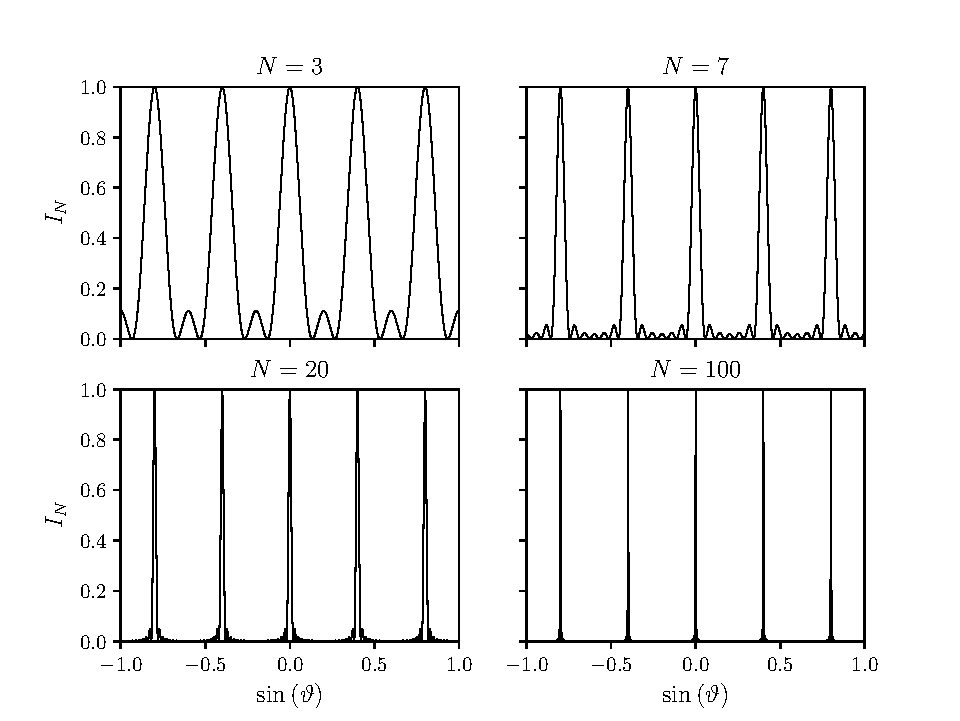
\includegraphics[scale=0.99]{Appendix-D/Figures/multi_slit_plots.pdf}%see intensity_plots.py
\caption[Normalized, far-field interference functions for $N$ sources]{Normalized, far-field interference functions for $N$ sources as a function of $\sin (\vartheta)$ with $\lambda / d = 0.4$.}\label{fig:multi_slit_plot}
\end{figure}
In these plots, it is seen that the number of primary fringes is the same as the double-slit experiment in \cref{fig:double_slit_plot}. 
Given by \cref{eq:fringes}, there are five of these fringes corresponding to a value of $\vartheta_{\text{max}}$ with $n = 0, \pm 1, \pm 2$. 
For $N > 2$, there also exist secondary fringes with maxima separated by points of zero intensity. 
From \cref{eq:N-slit_intensity}, this condition is for normal incidence is 
\begin{equation}\label{eq:fringe_min}
 \begin{split}
 \cos \left( N \Phi \right) = 1 &\implies N \Phi = 2 n \pi \\
 \Phi = \Phi^{\text{normal}} \equiv - k d \sin (\vartheta) &\implies \sin \left( \vartheta_{\text{min}} \right) = - \frac{n}{N} \frac{\lambda}{d} ,
 \end{split}
 \end{equation}
where $\Phi^{\text{normal}}$ is the multi-slit phase shift for this scenario of normal incidence. 
Seen in \cref{fig:multi_slit_plot}, the number of these minima increases with $N$, which causes the number of secondary maxima to increase while their intensities become suppressed. 
Simultaneously, the angular width of the main fringes decreases due to these closely spaced minima, especially as $N$ becomes very large. 

In the limit that $N \to \infty$, the structure can be treated as periodic with $K$ being the \emph{grating wave number} used in \cref{sec:grating_boundary}: 
\begin{equation}\label{eq:grating_number}
 K \equiv \frac{2 \pi}{d} .
 \end{equation}
This causes each fringe to be concentrated into an angular direction $\vartheta_{\text{max}}$ given by \cref{eq:fringes} for $n = 0, \pm 1, \pm 2$ and the secondary fringes vanish. 
The $N$ sources in this scenario start to behave like a diffraction grating, where far-field fringes (now referred to as \emph{diffracted orders}) propagate as planar waves. 
For an arbitrary $\lambda / d$ ratio, the \emph{diffracted angle}, $\vartheta_{\text{max}} \to - \beta_n$ from \cref{eq:fringes} is given by 
\begin{subequations}
\begin{equation}\label{eq:normal_incidence_orders}
 \sin \left( \beta_n \right) = \frac{n \lambda}{d} \quad \text{for } n = 0, \pm 1, \pm 2, \pm 3 \dotsc ,
 \end{equation}
which is a special case of the grating equation for normal incidence. 
For each order number, $n$, such that $- \pi / 2 < \Re \left[ \beta_n \right] < \pi /2$, \emph{propagating orders} exist in the far field. 
Otherwise, when $\abs{n \lambda / d} > 1$ the orders are \emph{evanescent} with $\Re \left[ \beta_n \right] \pm \pi / 2$ and $\Im \left[ \beta_n \right] \neq 0$. 

The expression in \cref{eq:normal_incidence_orders} can also be viewed in terms of wave numbers involving the grating periodicity along the $x$-direction and the $x$-component of the diffracted wave. 
That is, the diffracted wave vector has an $x$-component $k'_{x,n} \equiv k \sin \left( \beta_n \right)$ equal to an integer number of grating wave vectors:
\begin{equation}\label{eq:normal_incidence_orders_wave_number}
 k'_{x,n} = n K \quad \text{for } n = 0, \pm 1, \pm 2, \pm 3 \dotsc 
 \end{equation}
In other words, dispersion takes place in the direction orthogonal to the groove direction and to the grating normal (\emph{i.e.}, the $x$-axis in \cref{fig:double_slit_plot}). 
\end{subequations}
It can be gleaned from \cref{eq:normal_incidence_orders,eq:normal_incidence_orders_wave_number}  that for $\lambda$ characteristic of hard x-rays, diffraction is produced from $d$ on the order of atomic scales \cite{Bragg1913a,Compton35,Als-Nielsen11}. 
In this way, crystalline materials featuring regularly-spaced atoms (\emph{e.g.}, silicon shown in \cref{fig:crystal_structure}) produce x-ray diffraction patterns that can be used for a variety of applications including x-ray spectroscopy \cite{Giacconi79}. 
However, there is little versatility for crystal spectrometers in the soft x-ray band, where $\lambda$ is comparatively long and instead, custom diffraction gratings are better suited for the task.

\section{Off-Plane Geometry}\label{sec:off-plane_geo}
%%%%%%%%%%%%%%%%%%%%%%%%%%%%%%%%%%%%%%%%%--------------------------------------------------
The grazing-incidence requirement of soft x-rays [\emph{cf.\@} \cref{app:x-ray_materials}] requires generalizing the multi-slit interference scenario outlined in \cref{sec:slit_array} to include extra components to the phase shift $\Phi = - k \Delta s$ that arise from using oblique incidence angles in 3D geometries. 
To start, the incident plane wave can be imagined to have a wave vector $\mathbold{k}$ that is confined to the $x-y$ plane, but at an angle $\alpha$ as illustrated in the top panel of \cref{fig:oblique_off-plane}. 
Instead of $\mathbold{k} = k \mathbold{\hat{y}}$ as in \cref{fig:double_slit_experiment,fig:double_slit_experiment_approx}, the wave vector for this scenario is written as 
\begin{subequations}
\begin{equation}\label{eq:in-plane_wave_vector}
 \mathbold{k} = - k \left[ \sin (\alpha) \mathbold{\hat{x}} + \cos(\alpha) \mathbold{\hat{y}} \right] ,
 \end{equation}
so that the total path-length difference becomes $\Delta s = - d \left[ \sin (\beta_n) + \sin(\alpha) \right]$ in the far field, for $N \to \infty$. 
In this case, the diffraction pattern can be described two-dimensionally such that the incident ray is \emph{in-plane} with the orientations of all diffracted fringes. 
The multi-slit phase shift for this scenario is given by 
\begin{equation}\label{eq:in-plane_phase_shift}
 \Phi^{\text{in-plane}} = - k \Delta s = k d \left[ \sin (\beta_n) + \sin(\alpha) \right] = \Phi^{\text{normal}} + k d \sin(\alpha), 
 \end{equation}
where $\Phi^{\text{normal}} \equiv - k d \sin (\vartheta) \to k d \sin (\beta_n)$ is the phase shift for normal incidence [\emph{cf.\@} \cref{sec:slit_array,fig:double_slit_plot}]. 
\begin{figure}
 \hspace{-2cm}  
 \includegraphics[scale=0.85]{Appendix-D/Figures/diffraction_arc14.mps}
 \centering 
 \rule{\textwidth}{.4pt}
 \includegraphics[scale=0.85]{Appendix-D/Figures/diffraction_arc13.mps}
 \caption[Orientation of a representative wave vector for a generic oblique angle of incidence]{Orientation of a representative wave vector for a generic oblique angle of incidence. The top panel shows the vector confined to the $x-y$ plane, where in-plane diffraction occurs. The bottom panel shows the vector with a $z$-component, in which case off-plane diffraction occurs. The bottom panel appears the same as the top panel in projection when viewed directly down the $z$-axis.}\label{fig:oblique_off-plane}
 \end{figure}

This relation given by \cref{eq:in-plane_phase_shift} implies that with choice of large $\sin(\alpha)$, the phase shift is increased substantially. 
Noting that \cref{eq:normal_incidence_orders} in this case becomes 
\begin{equation}\label{eq:in-plane_orders}
 \sin \left( \alpha \right) + \sin \left( \beta_n \right) = \frac{n \lambda}{d} \quad \text{for } n = 0, \pm 1, \pm 2, \pm 3 \dotsc ,
 \end{equation}
the in-plane geometry under grazing incidence with $\sin(\alpha)$ approaching unity allows for large diffracted angles as compared to normal incidence for the same value of $d$. 
\end{subequations} 
This allows $d \gg \lambda$ provided that there is a very shallow angle of incidence confined to the $x-y$ plane as in \cref{fig:double_slit_plot} and the top panel of \cref{fig:oblique_off-plane}. 
For example, the soft x-ray reflection gratings on \emph{XMM-Newton}, which are designed for an in-plane geometry with $\alpha \approx 88.5^{\circ}$, have a groove spacing of $d \sim \SI{1.5}{\um}$ \cite{denHerder01}. 
On the other hand, \emph{critical angle transmission gratings} use $\alpha$ on the order of just a few degrees and in this case the aperture spacing is commonly $\SI{200}{\nm}$ \cite{Heilmann11}. 

In a more general scenario to that just described, the wave vector $\mathbold{k}$ has a $z$ component characterized by the angle $\gamma$ illustrated in the bottom panel of \cref{fig:oblique_off-plane} such that \cref{eq:in-plane_wave_vector} for the wave vector becomes [\emph{cf.\@} \cref{fig:grating_angles}] 
\begin{subequations}
\begin{equation}
 \mathbold{k} =  - k \left[ \sin (\alpha) \sin (\gamma) \mathbold{\hat{x}} + \cos(\alpha) \sin (\gamma) \mathbold{\hat{y}} - \cos (\gamma) \mathbold{\hat{z}} \right] ,
 \end{equation}
which will be shown to cause \emph{off-plane} diffraction [\emph{cf.\@} \cref{sec:grating_boundary}]. 
The multi-slit phase shift between the sources as observed in the far field is 
\begin{equation}\label{eq:off-plane_phase}
 \Phi^{\text{off-plane}} = - k \Delta s = k d \sin (\gamma) \left[ \sin (\beta_n) + \sin(\alpha) \right] = \sin (\gamma) \, \Phi^{\text{in-plane}}  
 \end{equation}
as a generalization of \cref{eq:in-plane_phase_shift}, which indicates a reduction relative to the in-plane case by a factor of $\sin (\gamma)$. 
This has the consequence that for extreme off-plane geometries with $\gamma$ of a few degrees, $d$ must be smaller than what it would be for a typical in-plane grazing incidence geometry [\emph{cf.\@} \cref{eq:inplane_limit,eq:offplane_limit}]. 
For example, off-plane gratings for soft x-rays currently under study commonly range from $\SI{400}{\nm}$ down to $\SI{160}{\nm}$ depending on the design of the spectrometer \cite{McEntaffer13,Miles18,McCurdy20,McCoy20}. 
This scenario of off-plane diffraction can also be described using framework for in-plane diffraction, where $\mathbold{k}$ is projected onto the the $x-y$ plane so that its magnitude, $\bar{k} \equiv k \sin (\gamma)$, can be thought of as an effective wave number with an increased wavelength, $\bar{\lambda} = \lambda \csc (\gamma)$. 
\end{subequations}

As the number of slits become very large and the fringes behave as collimated diffracted orders, equating $\Phi^{\text{off-plane}} = 2 n \pi$ with $n = 0, \pm 1, \pm 2, \pm 3 \dotsc$ gives the \emph{generalized grating equation}:
\begin{subequations}
\begin{equation}\label{eq:off-plane_incidence_orders}
 \sin \left( \alpha \right) + \sin \left( \beta_n \right) = \frac{n \lambda}{d \sin(\gamma)} \quad \text{for } n = 0, \pm 1, \pm 2, \pm 3 \dotsc 
 \end{equation}
Similar to \cref{eq:normal_incidence_orders_wave_number}, this can be expressed in terms of wave numbers [\emph{cf.\@} \cref{sec:reflected_diffracted}]: 
\begin{equation}\label{eq:off-plane_orders_wave_number}
  k'_{x,n} - k_x = n K \quad \text{for } n = 0, \pm 1, \pm 2, \pm 3 \dotsc ,
 \end{equation}
where $k'_{x,n} \equiv k \sin (\gamma) \sin(\beta_n)$ and $k_x \equiv - k \sin (\gamma) \sin(\alpha)$ so that it can be seen explicitly that grating dispersion takes places entirely in the $x$-direction (the \emph{grating-dispersion direction}).  
In this geometry, diffracted orders by definition have the following $y$-component to the wave vector: 
\begin{equation}
 k'_{y,n} = \pm \sqrt{k^2 - k'^2_{x,n} - k_z^2} \quad \text{with } k_z \equiv k \cos (\gamma) .
 \end{equation}
\end{subequations}
Propagating orders that correspond to those values of $n$ for which $k'_{y,n}$ is real lay on the surface of a cone with an opening angle of $2 \gamma$ while still being equally spaced along the $x$-axis \cite{Neviere78}. 
\begin{figure}
 \centering
 \includegraphics[scale=0.85]{Appendix-D/Figures/diffraction_arc15.mps}
 \caption{Geometry for a transmission grating producing conical diffraction}\label{fig:conical_transmission}
 \end{figure}
This is visualized for the case of a transmission grating in \cref{fig:conical_transmission}, where the $0^{\text{th}}$ order passes straight through the structure while any given propagating order intersects with the circle drawn in the figure. 

A reflection grating in this conical geometry is shown in \cref{fig:conical_reflection}, where the $0^{\text{th}}$ order is equivalent to the reflected beam from a mirror and all propagating orders lay on the upper-half of the cone. 
\begin{figure}
 \centering
 \includegraphics[scale=0.85]{Appendix-D/Figures/diffraction_arc16.mps}
 \caption{Geometry for a reflection grating producing conical diffraction}\label{fig:conical_reflection}
 \end{figure}
At a distance $L \gg (N-1) d$ away from the grating for either case, the radius of this circle is $r = L \sin (\gamma)$ [\emph{cf.\@} \cref{eq:arc_radius}] and the $x$-distance between the $n^{\text{th}}$ and $0^{\text{th}}$ orders is given by 
\begin{subequations}
\begin{equation}
 x_n = r \left[ \sin \left( \alpha \right) + \sin \left( \beta_n \right) \right] .
 \end{equation}
Using \cref{eq:off-plane_incidence_orders} this becomes [\emph{cf.\@} \cref{eq:linear_dispersion}] 
\begin{equation}\label{eq:dispersion}
 x_n = \frac{n \lambda L}{d} ,
 \end{equation}
\end{subequations}
as labeled in \cref{fig:conical_transmission,fig:conical_reflection}. 
This shows that no matter the incidence angle, the linear dispersion between propagating orders on an imaging detector a distance $L$ away from the grating is proportional to $\lambda /d$ as well as $\abs{n}$. 

\section{On Spectral Resolving Power}\label{sec:resolving_power}
%%%%%%%%%%%%%%%%%%%%%%%%%%%%%%%%%%%%%%%%%--------------------------------------------------
In spectroscopy, the purpose of a diffraction grating is to disperse white light according to color so that the intensity of its constituent wavelength components can be measured and plotted as a spectrum. 
From \cref{eq:off-plane_incidence_orders}, this is based on the principle that a monochromatic plane wave incident on a barrier with $N$ infinitesimal slits produces a number of primary fringe maxima depending on the ratio $\lambda /d$; in the limit that $N$ is very large, these maxima become diffracted orders that are observed as plane waves in the far field [\emph{cf.\@} \cref{sec:slit_array}]. 
On a screen a distance $L \gg (N - 1) d$ away from a grating with $N$ slits or grooves, the $n^{\text{th}}$ diffracted order exists at a position relative to $0^{\text{th}}$ order given by \cref{eq:dispersion}. 
The secondary fringes are separated by a distance $\Delta x = L \lambda / N d$ [\emph{cf.\@} \cref{eq:fringe_min}], which implies that each primary fringe has a width $\Delta x$ on the screen. 
Based on these considerations alone, the spectral resolving power, $\mathscr{R}$, of such a grating is \cite{Loewen97} 
\begin{equation}\label{eq:diffraction_limit_res}
 \frac{\lambda}{\Delta \lambda} = \abs{\frac{x_n}{\Delta x}} = \abs{n} N ,
 \end{equation}
which applies only to a \emph{diffraction-limited} scenario, where all other aberrations arising from optical imperfections can be neglected. 
Essentially, this states that the maximum $\mathscr{R}$ that can possibly be attained is dependent on the number of slit sources and that spectra become increasingly easier to resolve as the magnitude of the order number increases. 
However, \cref{eq:diffraction_limit_res} is also dependent on the angles of incidence, which can be seen using \cref{eq:off-plane_incidence_orders} to write 
\begin{equation}
 \abs{n} = \sin \left( \gamma \right) \abs{\sin \left( \alpha \right) + \sin \left( \beta_n \right)} \frac{d}{\lambda}
 \end{equation} 
so that \cref{eq:diffraction_limit_res} becomes 
\begin{subequations}
\begin{equation}\label{eq:diffraction_limit_res_angle}
 \frac{\lambda}{\Delta \lambda} = \sin \left( \gamma \right) \abs{\sin \left( \alpha \right) + \sin \left( \beta_n \right)} \frac{N d}{\lambda} ,
 \end{equation}
which states that higher $\mathscr{R}$ is achieved with large angles of incidence and diffraction \cite{Loewen97}. 
The maximum $\mathscr{R}$ attainable for a grating with $N$ perfectly spaced apertures is then 
\begin{equation}\label{eq:diffraction_limit_res_angle_max}
 \frac{\lambda}{\Delta \lambda} = \frac{2 N d}{\lambda} ,
 \end{equation}
\end{subequations}
where $N d$ is the ruled width of the grating. 

As a simple example that demonstrates the concept of diffraction-limited $\mathscr{R}$, it is supposed that collimated white light composed of representative red, green and blue wavelengths in equal parts is normally incident on the barrier drawn in \cref{fig:double_slit_plot}, but with $N$ regularly-spaced, infinitesimal slits. 
Shown in \cref{fig:multi_slit_plot_color}, each color is dispersed by a different amount proportional to the ratio $\lambda / d$ so that effectively, a spectrum is produced around each primary fringe maximum for $n = \pm 1, \pm 2$.  
\begin{figure}
\centering
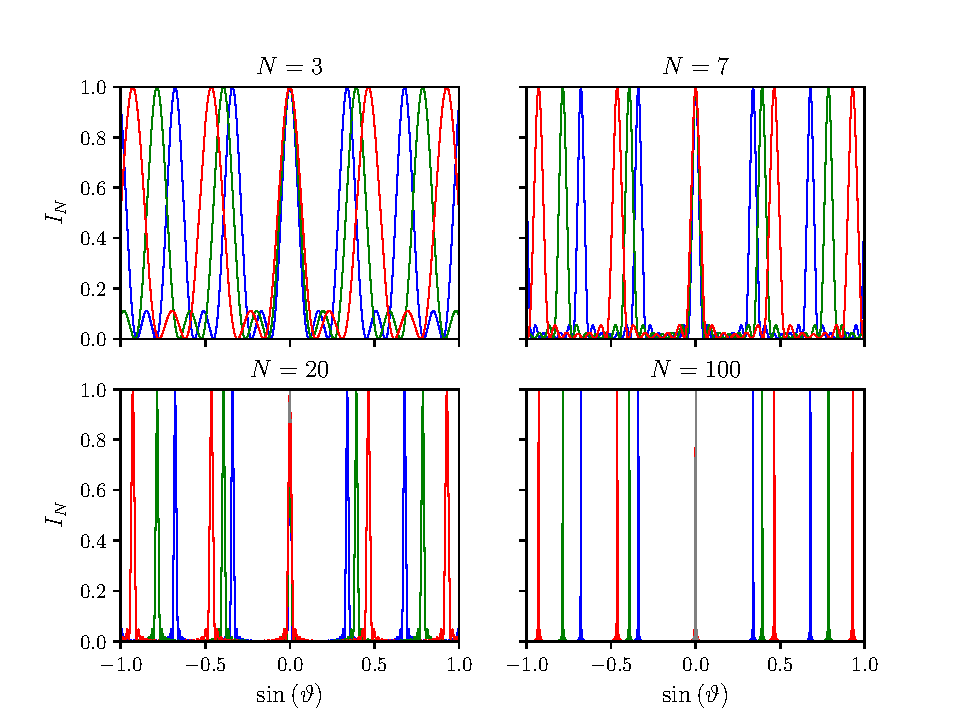
\includegraphics[scale=0.99]{Appendix-D/Figures/multi_slit_plots_color.pdf}
\caption[Far-field interference of polychromatic light for $N$ sources]{Far-field interference for $N$ sources as a function of $\sin (\vartheta)$ for wavelengths corresponding to red ($\lambda = \SI{650}{\nm}$), green ($\lambda = \SI{550}{\nm}$) and blue ($\lambda = \SI{475}{\nm}$) with $d = \SI{1.4}{\micro\metre}$.}\label{fig:multi_slit_plot_color}
\end{figure}  
It is clear from the figure that unless $N$ is large enough, these fringes overlap with each other and hence the colors cannot be distinguished through grating dispersion. 
Although only a modest value of $N$ is needed to distinguish between the red, green and blue wavelengths in the case of \cref{fig:multi_slit_plot_color}, generally a very large number of slits is needed to separate colors closer together in wavelength. 
However, as the number of these fringes increases with decreasing $\lambda / d$, inevitably there will be some spectral overlap. 
For this reason, diffracted orders generally need to be separated for useful spectra to be extracted. 
\begin{figure}
\centering
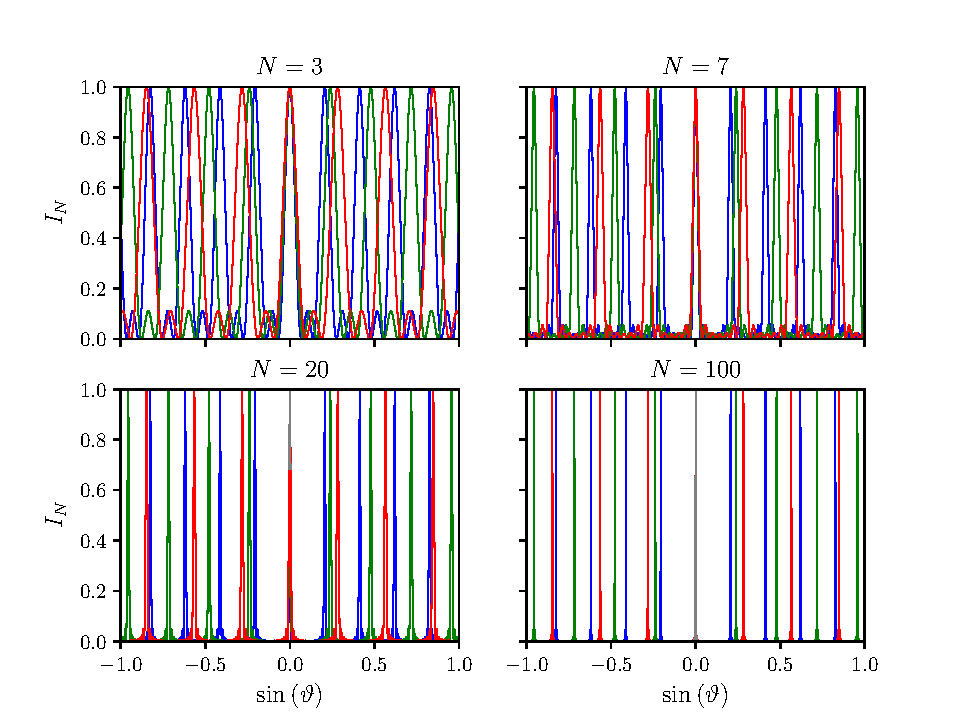
\includegraphics[scale=0.99]{Appendix-D/Figures/multi_slit_plots_color_confusion.pdf}
\caption[Far-field interference of polychromatic light for $N$ sources with order confusion]{Far-field interference for $N$ sources as a function of $\sin (\vartheta)$ for wavelengths corresponding to red ($\lambda = \SI{650}{\nm}$), green ($\lambda = \SI{550}{\nm}$) and blue ($\lambda = \SI{475}{\nm}$) with $d = \SI{2.3}{\micro\metre}$, demonstrating the concept of order confusion.}\label{fig:multi_slit_plot_color_confusion}
\end{figure}
This is demonstrated in \cref{fig:multi_slit_plot_color_confusion}, where the red, green and blue wavelengths from \cref{fig:multi_slit_plot_color} are dispersed by $N$ slits with a different value for $d$.

Spectral resolving power can also be treated using the framework of \emph{Fraunhofer diffraction} such that an array of $N$ in-phase, infinitesimal slits, each spaced by the same distance $d$, can be described as a sum of \emph{Dirac delta functions}:\footnote{A Dirac delta function is defined as 
\begin{equation*}
\delta_D \left( x \right) \equiv
   \begin{cases}
     \infty, & \text{if}\ x = 0 \\
     0, & \text{if}\ x \neq 0 .
   \end{cases} 
\end{equation*}}
\begin{subequations}
\begin{equation}\label{eq:amplitude_dirac_finite}
 \mathcal{A} (x) = \mathcal{A}_0 \sum_{m=1}^{N} \delta_D \left( \frac{x}{d} - m \right) .
 \end{equation}
Taking the Fourier transform and using the exponential-sum formula given by \cref{eq:exp_sum} with $\Phi \to - k'_x d$ yields 
\begin{align}
 \begin{split}\label{eq:DC_FT}
 \mathcal{A} \left( k'_x \right) &= \mathcal{A}_0 \, d \int_{-\infty}^{\infty} \sum_{m=1}^{N} \delta_D \left( x - m d \right) \mathrm{e}^{-i k'_x x} \dd{x} \\
 &= \mathcal{A}_0 \, d \sum_{m=1}^{N} \mathrm{e}^{-i k'_x m d} = \mathrm{e}^{-i k'_x d} \frac{1 - \mathrm{e}^{- i N k'_x d}}{1 - \mathrm{e}^{- i k'_x d}} .
 \end{split}
 \end{align}
The corresponding far-field interference pattern is the squared norm of this function: 
\begin{equation}
 I_N = \norm{\mathcal{A} \left( k'_x \right)}^2 = \mathcal{A}_0^2 \frac{1 - \cos \left( N k'_x d \right)}{1 - \cos \left( k'_x d \right)} ,
 \end{equation}
\end{subequations}
which is equivalent to the multi-slit intensity function given by \cref{eq:N-slit_intensity}. 
This indicates that a grating with a perfect but finite slit periodicity is associated with diffraction-limited $\mathscr{R}$ [\emph{cf.\@} \cref{eq:diffraction_limit_res,eq:diffraction_limit_res_angle,eq:diffraction_limit_res_angle_max}]. 

In the limit that $N \to \infty$, \cref{eq:amplitude_dirac_finite} becomes 
\begin{equation}\label{eq:amplitude_dirac}
 \mathcal{A} (x) = \mathcal{A}_0 \sum_{n=-\infty}^{\infty} \delta_D \left( \frac{x}{d} - n \right) \equiv \mathcal{A}_0 \, \Sha \left( \frac{x}{d} \right) = \mathcal{A}_0 \, d \, \Sha \left( x \right) ,
 \end{equation}
where $\Sha \left( x \right)$ is known as the \emph{Dirac comb}. 
The Fourier transform of \cref{eq:amplitude_dirac} is
\begin{subequations}
\begin{align}\label{eq:eq:amplitude_dirac_FT}
 \begin{split}
 \mathcal{A} \left( k'_x \right) &= \mathcal{A}_0 \int_{-\infty}^{\infty} \Sha \! \left( \frac{x}{d} \right) \mathrm{e}^{-i k'_x x} \dd{x} \\
 &= \mathcal{A}_0 \int_{-\infty}^{\infty} \sum_{n=-\infty}^{\infty} \delta_D \left( \frac{x}{d} - n \right) \mathrm{e}^{-i k'_x x} \dd{x} = \mathcal{A}_0 \sum_{n=-\infty}^{\infty} \mathrm{e}^{-i k'_x n d} , 
 \end{split}
 \end{align}
which is recognized up to a factor of $2 \pi / d \equiv K$ as the Fourier-series expansion of a Dirac comb:
\begin{equation}\label{eq:sha_FS}
 \Sha \! \left( - \frac{k'_x}{2 \pi} \right) \equiv d \sum_{n=-\infty}^{\infty} \mathrm{e}^{-i k'_x n d} = 2 \pi \, \Sha \! \left( k'_x \right)  
 \end{equation}
so that 
\begin{equation}\label{eq:sha_FT}
 \int_{-\infty}^{\infty} \Sha \! \left( \frac{x}{d} \right) \mathrm{e}^{-i k'_x x} \dd{x} = \Sha \! \left( \frac{k'_x}{K} \right) .
 \end{equation}
\end{subequations}
Here, $\mathcal{A} \left( k'_x \right)$ is the far-field amplitude of a grating with $\mathscr{R} \to \infty$, where each diffracted order is associated with a singular value of $k'_x$ as described by the sum of Dirac delta functions. 

In practice, $N$ can be considered to approach infinity for an x-ray reflection of substantial size.  
The silicon grating with $d \lessapprox \SI{160}{\nm}$ described in \cref{sec:crystal_etching}, for example, has $N \gtrapprox \num{468750}$ so that diffraction-limited $\mathscr{R}$ is on the order of \num{100000} or more by \cref{eq:diffraction_limit_res}. 
On the other hand, the spectral resolving power of an x-ray reflection grating, is limited (typically to a few thousand) by how well the radially-ruled profile of the grating grooves matches the focal length of a Wolter-I telescope [\emph{cf.\@} \cref{sec:grating_tech_intro}]. 
While beamline testing for $\mathscr{R}$ is beyond the scope of this dissertation, it is noted that an imperfect $\mathscr{R}$ effectively serves to broaden the angular spread of each propagating order so that, in principle, the total flux associated with each diffracted beam is unaffected. 
Because of this, $\mathscr{R} \to \infty$ with $N \to \infty$ is assumed for the examination of scalar diffraction efficiency in \cref{sec:amplitude_phase}. 

\section{Groove Shape Impact on Diffraction Efficiency}\label{sec:amplitude_phase}
%%%%%%%%%%%%%%%%%%%%%%%%%%%%%%%%%%%%%%%%%--------------------------------------------------
A diffraction grating broadly can be considered to be any sort of structure that causes an incident wave to undergo periodic shifts in amplitude, phase, or possibly both, across its surface. 
The example of water waves passing through a set of evenly-spaced obstacles is analogous to a transmission grating for electromagnetic radiation that features a finely-pitched periodic array of absorbing slabs. %mentioned previously
In the simplest of scenarios, such an optical device functions as an \emph{amplitude grating}, where, by the Huygens-Fresnel principle, the point sources of wavelength $\lambda$ that constitute its surface can be regarded to vary in amplitude alone. 
According to the framework of Fraunhofer diffraction [\emph{cf.\@} \cref{sec:resolving_power}], the far-field interference pattern then is the Fourier transform of this periodic amplitude function \cite{Born80}. 
That is, if an array of slits can be described with an amplitude function $\mathcal{A} (x)$, then the Fourier transform is a function of the $x$-component of the diffracted wave vector in the far field with $k'_x \equiv k \sin \left( \gamma \right) \sin \left( \beta_n \right)$: 
\begin{subequations}
\begin{equation}
 \mathcal{A} \left( k'_x \right) = \int_{-\infty}^{\infty} \mathcal{A} (x) \, \mathrm{e}^{-i k'_x x} \dd{x} ,
 \end{equation}
so that taking the inverse-Fourier transform recovers $\mathcal{A} (x)$: 
\begin{equation}\label{eq:amplitude_Fourier}
 \mathcal{A} (x) = \frac{1}{2 \pi} \int_{-\infty}^{\infty} \mathcal{A} \left( k'_x \right) \mathrm{e}^{i k'_x x} \dd{k'_x} .
 \end{equation}
\end{subequations}

On the other hand, a reflection grating realized as a mirror with regularly-spaced grooves etched into its surface (also described as a \emph{surface-relief grating}) may not provide any variation in amplitude at all. 
Rather, as light traverses the depth of the grooves and reflects back under ideal conditions, the net result is a periodic phase shift and the surface can be thought of as a \emph{phase grating} that determines the far-field interference pattern.  
To study this, a more general version of \cref{eq:amplitude_Fourier} is defined as the grating \emph{transmittance function} \cite{Sanchez-Lopez09,Harvey19,Casini14}:
\begin{subequations}
\begin{equation} \label{eq:grating_transmittance}
 G (x) \equiv \mathcal{A} (x) \mathrm{e}^{i \Phi (x)} = \frac{1}{2 \pi} \int_{-\infty}^{\infty} G \left( k'_x \right) \mathrm{e}^{i k'_x x} \dd{k'_x} 
 \end{equation}
with a Fourier transform describing the far-field interference pattern given by 
\begin{equation}
 G \left( k'_x \right) = \int_{-\infty}^{\infty} G (x) \, \mathrm{e}^{-i k'_x x} \dd{x} .
 \end{equation}
If $G(x)$ is periodic with $G (x+d) = G (x)$, it can be expressed as a Fourier series: 
\begin{equation} \label{eq:grating_transmittance_series}
 G (x) = \sum_{n=-\infty}^{\infty} G_n \mathrm{e}^{i n K x} ,
 \end{equation}
where $K \equiv 2 \pi /d$ [\emph{cf.\@} \cref{eq:grating_number}] and the Fourier coefficients are
\begin{equation} \label{eq:transmit_fourier_coeff}
 G_n = \frac{1}{d} \int_{0}^{d} G \left( x \right) \mathrm{e}^{- i n K x} \dd{x} \quad \text{for } n = 0, \pm 1, \pm 2, \pm 3 \dotsc
 \end{equation} 
\end{subequations}
Far-field intensity in the $n^{\text{th}}$ diffracted order, $\mathcal{I}_n$, as is it passes through a plane parallel to the grating surface depends on the following projection of Poynting's vector:
\begin{equation}\label{eq:order_intensity_scalar}
 \mathcal{I}_n = \mathbold{S}_n \cdot \mathbold{\hat{y}} \propto \sin \left( \gamma \right) \cos \left( \beta_n \right) \norm{G_n}^2 ,
 \end{equation}
where $\mathbold{S}_n$ describes the directional energy flux of the $n^{\text{th}}$ propagating order. 

The assumption of $G (x+d) = G (x)$ for all $x$ implies a grating with $\mathscr{R} \to \infty$ so that in this case, the form of $G (x)$ only impacts diffraction efficiency [\emph{cf.\@} \cref{sec:resolving_power}]. 
Although the interaction of the incident wave with the grating structure is not treated under this framework, its intensity can be taken as $\mathcal{I}_{\text{inc}} \propto \sin \left( \gamma \right) \cos \left( \alpha \right)$ in analogy to \cref{eq:transmit_fourier_coeff} so that scalar diffraction efficiency is defined as 
\begin{equation}\label{eq:scalar_efficiency}
 \mathscr{E}_n \equiv \frac{\mathcal{I}_n}{\mathcal{I}_{\text{inc}}} \propto \frac{\cos \left( \beta_n \right)}{\cos \left( \alpha \right)} \norm{G_n}^2 .
 \end{equation}
Approximate behavior for \emph{relative diffraction efficiency} can be gleaned using \cref{eq:scalar_efficiency}, where the constant of proportionality is determined from requiring that $\sum_n \mathscr{E}_n = 1$ for all $n$ corresponding to propagating orders [\emph{cf.\@} \cref{sec:rel_eff_perf}]. 
In the discussion that follows, the efficiency behavior of common groove shapes are considered below with emphasis on phase gratings, where a function $\Phi (x+d) = \Phi (x)$ is used to describe surface-relief reflection gratings with various groove profiles. 

To formulate descriptions for amplitude and phase gratings, an array of $N \to \infty$ infinitesimal slits given by \cref{eq:amplitude_dirac} with $\mathcal{A} (x+d) = \mathcal{A} (x)$ is again considered. 
Inserting \cref{eq:amplitude_dirac} as $G(x)$ with $\Phi (x) = 0$ into \cref{eq:transmit_fourier_coeff} shows that the amplitude of each diffracted order in the far field is identical:
\begin{align} 
 \begin{split}\label{eq:amplitude_fourier_coeff}
 G_n &= \frac{\mathcal{A}_0}{d} \int_{0}^{d} \Sha \left( \frac{x}{d} \right) \mathrm{e}^{- i n K x} \dd{x} = \mathcal{A}_0 \int_{0}^{d} \sum_{m=-\infty}^{\infty} \delta_D \left( x - m d \right) \mathrm{e}^{- i n K x} \dd{x} \\
 &= \mathcal{A}_0 \int_{0}^{d} \delta_D \left( x - d \right) \mathrm{e}^{- i n K x} \dd{x} = \mathcal{A}_0 \mathrm{e}^{- i n \left( 2 \pi \right)} = \mathcal{A}_0 ,
 \end{split}
 \end{align} 
which is the same result obtained from \cref{eq:DC_FT} and the multi-slit interference function given by \cref{eq:N-slit_intensity} in the limit that $N \to \infty$. 
\begin{figure}
 \centering
 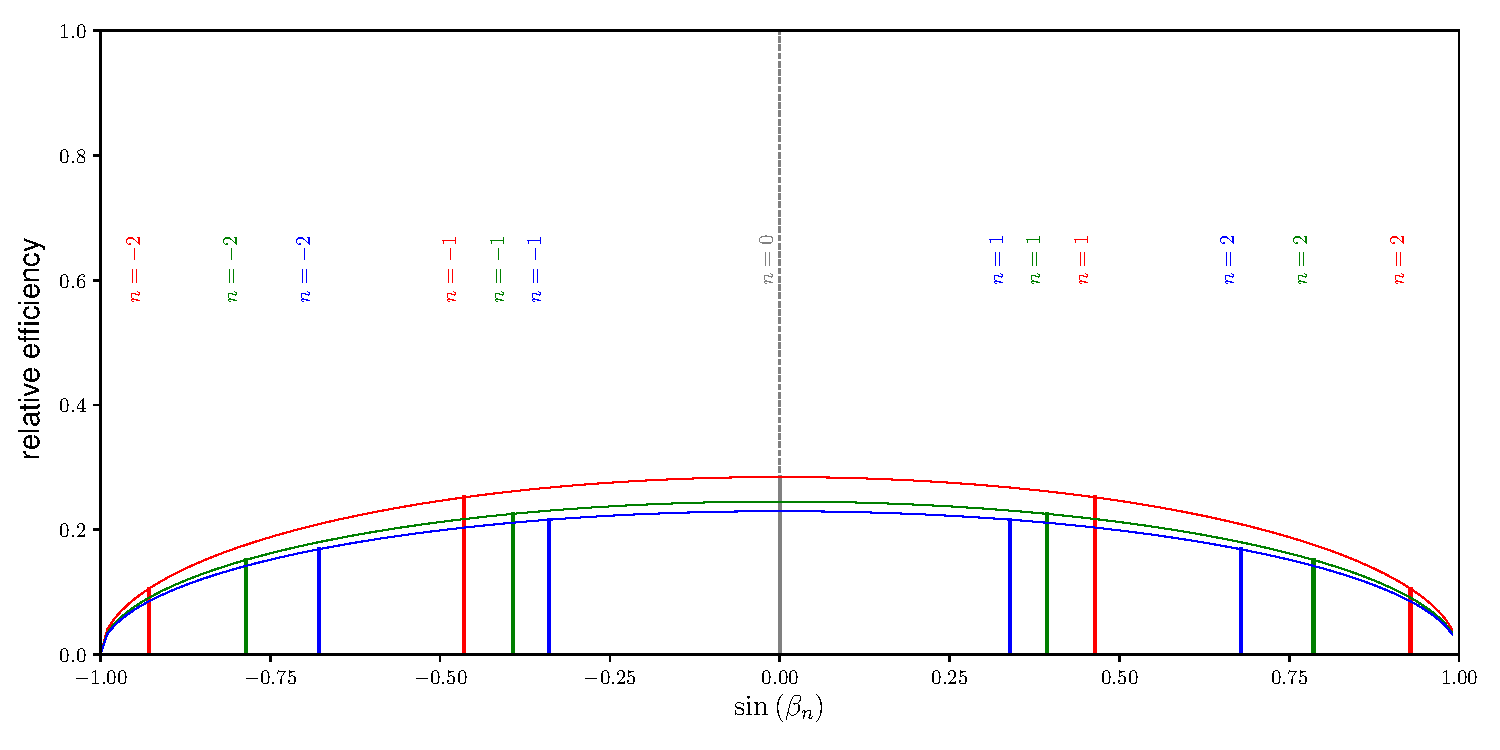
\includegraphics[scale=0.62]{Appendix-D/Figures/dirac_amplitude.pdf}
 \caption[Relative efficiency of a Dirac-comb amplitude grating.]{Relative efficiency of a Dirac-comb amplitude grating at normal incidence with $\lambda / d$ for red, green and blue.}\label{fig:dirac_amplitude}
 \end{figure} 
Relative diffraction efficiency, $\mathscr{E}_n$, in this case is modulated only by the trigonometric factors involving $\beta_n$ and $\alpha$ that appear in \cref{eq:scalar_efficiency} such that for $\alpha = 0$,
\begin{equation}
 \mathscr{E}_n \propto \cos \left( \beta_n \right) = \sqrt{1 - \left( \frac{n \lambda}{d} \right)^2} ,
 \end{equation}
which is plotted as relative efficiency in \cref{fig:dirac_amplitude} for three values of $\lambda / d$ that are representative of red, green and blue wavelengths [\emph{cf.\@} \cref{fig:multi_slit_plot_color}]. 
Unlike the Dirac comb [\emph{cf.\@} \cref{eq:amplitude_dirac,eq:amplitude_fourier_coeff}], real gratings have apertures with finite size or more generally, apertures where amplitude $\mathcal{A} (x)$ and phase $\Phi (x)$ vary across the periodic distance $d$, which results in a set of $G_n$ that vary between diffracted orders.  
The Dirac comb, however, can be viewed as a descriptor for the locations of diffracted order and it can be convolved with the diffraction pattern from a single slit to describe a grating with a finite aperture \cite{Loewen97,DeRoo16thesis}. 
Using a similar approach, the Fourier components for square wave, sinusoidal and sawtooth transmittance functions with $G (x+d) = G (x)$ are described in \cref{eq:square_principle,sec:sinusoid_principle,sec:sawtooth_principle}. 
Each example, as in \cref{fig:dirac_amplitude}, uses $\lambda =$~\SIlist{650;550;475}{\nm} for red, green and blue, respectively, with a groove spacing of $d = \SI{1.4}{\micro\metre}$. 
While these examples explicitly assume in-plane diffraction with $\sin \left( \gamma \right) = 1$, the more general off-plane case can recovered by substituting $\lambda \to \bar{\lambda} \equiv \lambda \csc \left( \gamma \right)$ [\emph{cf.\@} \cref{sec:off-plane_geo}]. 

\subsection{The Square Wave}\label{eq:square_principle}
%%%%%%%%%%%%%%%%%%%%%%%%%%%%%%%%%%%%%%%%%--------------------------------------------------
The first example to consider is a binary amplitude grating with a slit width $\mathscr{W}$, which is not assumed to be small compared to $\lambda$ as in the case of the Dirac comb. 
This parameter $\mathscr{W}$ sets the duty cycle, $\mathscr{W}/d$, of the piece-wise transmittance function for a square wave: 
\begin{subequations}
\begin{equation}
    G (x) = 
                \begin{cases}
                  \mathcal{A}_0 , &\quad \text{for } 0 < x \leq \mathscr{W} \\
                  0 , &\quad \text{for } \mathscr{W} < x \leq d ,
                \end{cases}
 \end{equation}
where \cref{eq:transmit_fourier_coeff} gives the following Fourier coefficients: 
\begin{equation}\label{eq:G_terms_square}
 G_n = \frac{\mathcal{A}_0}{d} \int_0^{\mathscr{W}} \mathrm{e}^{- i n K x} \dd{x} = \frac{i \mathcal{A}_0}{2 n \pi} \left( \mathrm{e}^{- i n K \mathscr{W}} - 1 \right) \quad \text{for } n = 0, \pm 1, \pm 2, \pm 3 \dotsc
 \end{equation}
Physically, this describes the behavior of a transmission grating featuring an array of absorbing slabs with scalar diffraction efficiency [\emph{cf.\@} \cref{eq:scalar_efficiency}] given by 
\begin{align}\label{eq:binary_amplitude_intensity}
 \begin{split}
 \mathscr{E}_n &\propto \frac{\cos \left( \beta_n \right)}{\cos \left( \alpha \right)} \norm{G_n}^2 \\
 \text{with} \quad \norm{G_n}^2 &\propto \frac{1}{2} \left( \frac{1}{n \pi} \right)^2 \left[ 1 - \cos \left( n K \mathscr{W} \right) \right] = \left( \frac{\mathscr{W}}{d} \right)^2 \sinc^2 \left( \frac{n \pi \mathscr{W}}{d} \right) ,
 \end{split}
\end{align}
\end{subequations}
where $\sinc (x) \equiv \sin(x) / x$ is the \emph{sinc function} [\emph{cf.\@} \cref{fig:sinc_squared}]. 
This shows that the intensity of propagating orders is dependent on the the ratio $n \mathscr{W} / d$ such that when it is an integer, intensity reaches zero. 

For example, a grating with a \SI{50}{\percent} duty cycle with $\mathscr{W} = d/2$ has all even orders other than $n=0$ vanish since $\norm{G_n}^2 \propto \sinc^2 \left( n \pi / 2 \right)$ for a fixed geometry; a \SI{25}{\percent} duty cycle with $\mathscr{W} = d/4$ yields $\norm{G_n}^2 \propto \sinc^2 \left( n \pi / 4 \right)$ and therefore every $4^{\text{th}}$ order is suppressed. 
\begin{figure}
 \centering
 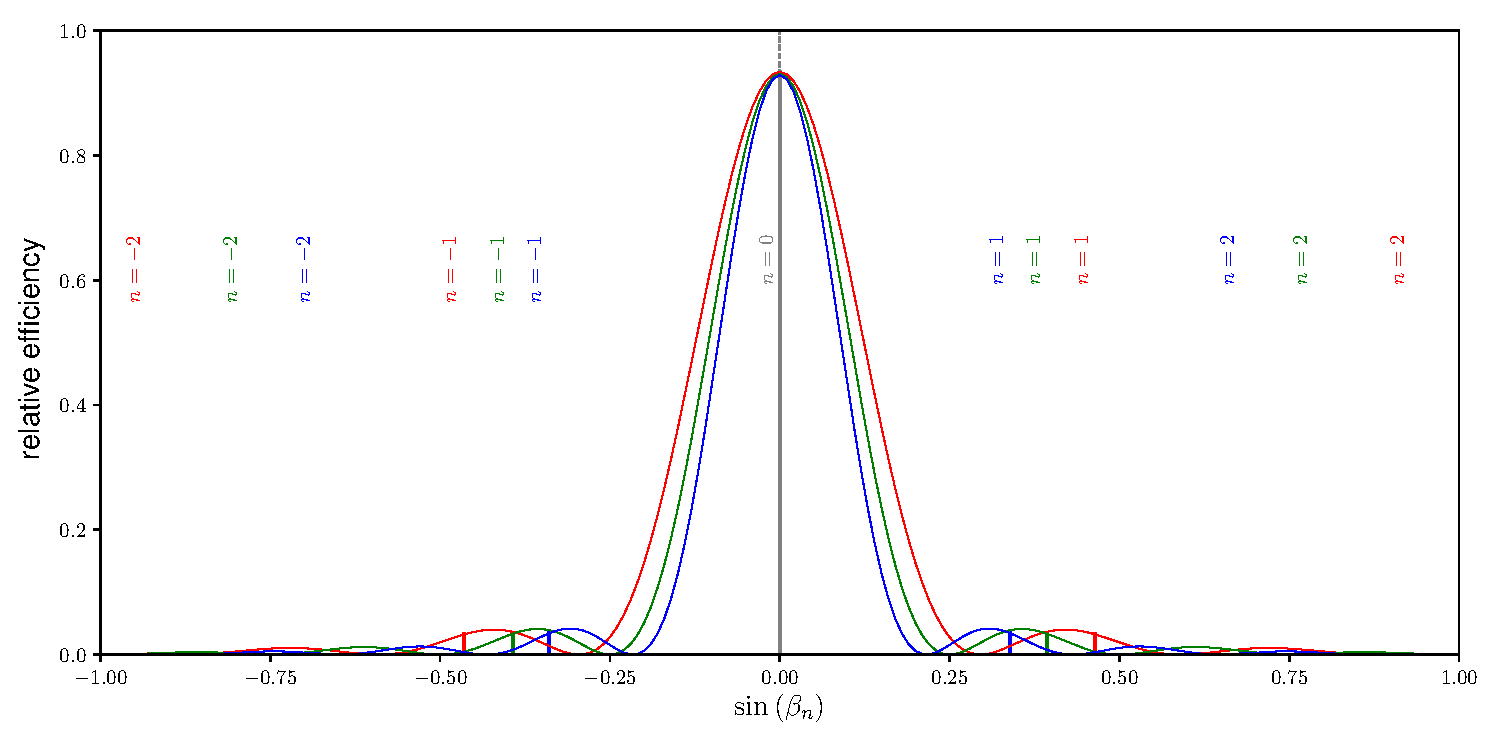
\includegraphics[scale=0.62]{Appendix-D/Figures/square_amplitude.pdf}
 \caption[Relative efficiency of a square-wave amplitude grating.]{Relative efficiency of a $\mathscr{W}/d = \SI{50}{\percent}$ square-wave amplitude grating at normal incidence with $\lambda / d$ for red, green and blue.}\label{fig:square_amplitude}
 \end{figure} 
Relative efficiency for a grating at normal incidence with $\mathscr{W} = d/2$ is plotted in \cref{fig:square_amplitude}, where it is seen that propagating orders with $n= \pm 2$ have $\mathscr{E}_n \approx 0$ as a result of $\mathscr{W}/d = \SI{50}{\percent}$. % a \SI{50}{\percent} duty cycle. 
In the figure, it is also seen that $\mathscr{E}_n$ for $n= \pm 1$ comprise a small percentage of the total efficiency. 
While this can be improved with smaller $\mathscr{W}/d$, efficiency is ultimately spread relatively evenly amongst unsuppressed propagating orders. 

A binary phase grating can be taken to represent a reflection grating used near normal incidence, where radiation picks up a phase shift $\Phi_g$ as radiation reflects from the the top and bottom of rectangular grooves\footnote{$\Phi_g$ is not to be confused with the multi-slit phase shift, $\Phi^{\text{off-plane}}$, given by \cref{eq:off-plane_phase}.} of width $\mathcal{W}$ and depth $h_0$. 
For an in-plane geometry, this phase shift from the groove facet can be written explicitly as\footnote{However, it should be noted that if radiation illuminates significant portions of the groove sidewalls, then this analysis does not hold.}
\begin{equation}\label{eq:laminar_phase}
 \Phi_g = \frac{2 \pi}{\lambda} h_0 \left[ \cos \left( \alpha \right) + \cos \left( \beta_n \right) \right] . 
 \end{equation}
With amplitude constant everywhere, a binary phase grating can be described using
\begin{subequations}
\begin{equation}
    G (x) = 
                \begin{cases}
                  \mathcal{A}_0 \mathrm{e}^{i \Phi_g} , &\quad \text{for } 0 < x \leq \mathscr{W} \\
                  \mathcal{A}_0 , &\quad \text{for } \mathscr{W} < x \leq d 
                \end{cases}
 \end{equation}
with Fourier coefficients coming out to
\begin{align}\label{eq:G_terms_square_phase}
 \begin{split}
 G_n &= \frac{\mathcal{A}_0}{d} \left( \mathrm{e}^{i \Phi_g} \int_0^{\mathscr{W}} \mathrm{e}^{- i n K x} \dd{x} + \int_{\mathscr{W}}^d \mathrm{e}^{- i n K x} \dd{x} \right) \\
 &= \frac{i \mathcal{A}_0}{2 n \pi} \left( \mathrm{e}^{i \Phi_g} - 1 \right) \left( \mathrm{e}^{- i n K \mathscr{W}} - 1 \right) \quad \text{for } n = 0, \pm 1, \pm 2, \pm 3 \dotsc  
 \end{split}
 \end{align}
so that the scalar diffraction efficiency is  
\begin{align}\label{eq:binary_phase_intensity}
 \begin{split}
 \mathscr{E}_n &\propto \frac{\cos \left( \beta_n \right)}{\cos \left( \alpha \right)} \norm{G_n}^2 \\
 \text{with} \quad \norm{G_n}^2 &\propto \left( \frac{1}{n \pi} \right)^2 \left[ 1 - \cos \left( n K \mathscr{W} \right) \right] \left[ 1 - \cos \left( \Phi_g \right) \right] \\
 &= \left( \frac{\mathscr{W} \Phi_g}{d} \right)^2 \sinc^2 \left( \frac{n \pi \mathscr{W}}{d} \right) \sinc^2 \left( \frac{\Phi_g}{2} \right) .
 \end{split}
 \end{align}
\end{subequations}
Therefore, similar to the results obtained from the amplitude amplitude grating considered above given by \cref{eq:binary_amplitude_intensity}, it is evident from \cref{eq:binary_phase_intensity} that the intensity of diffracted orders in this case is dependent on $n \mathscr{W} / d$ as well as $\Phi_g / 2 \pi$. 
\begin{figure}
 \centering
 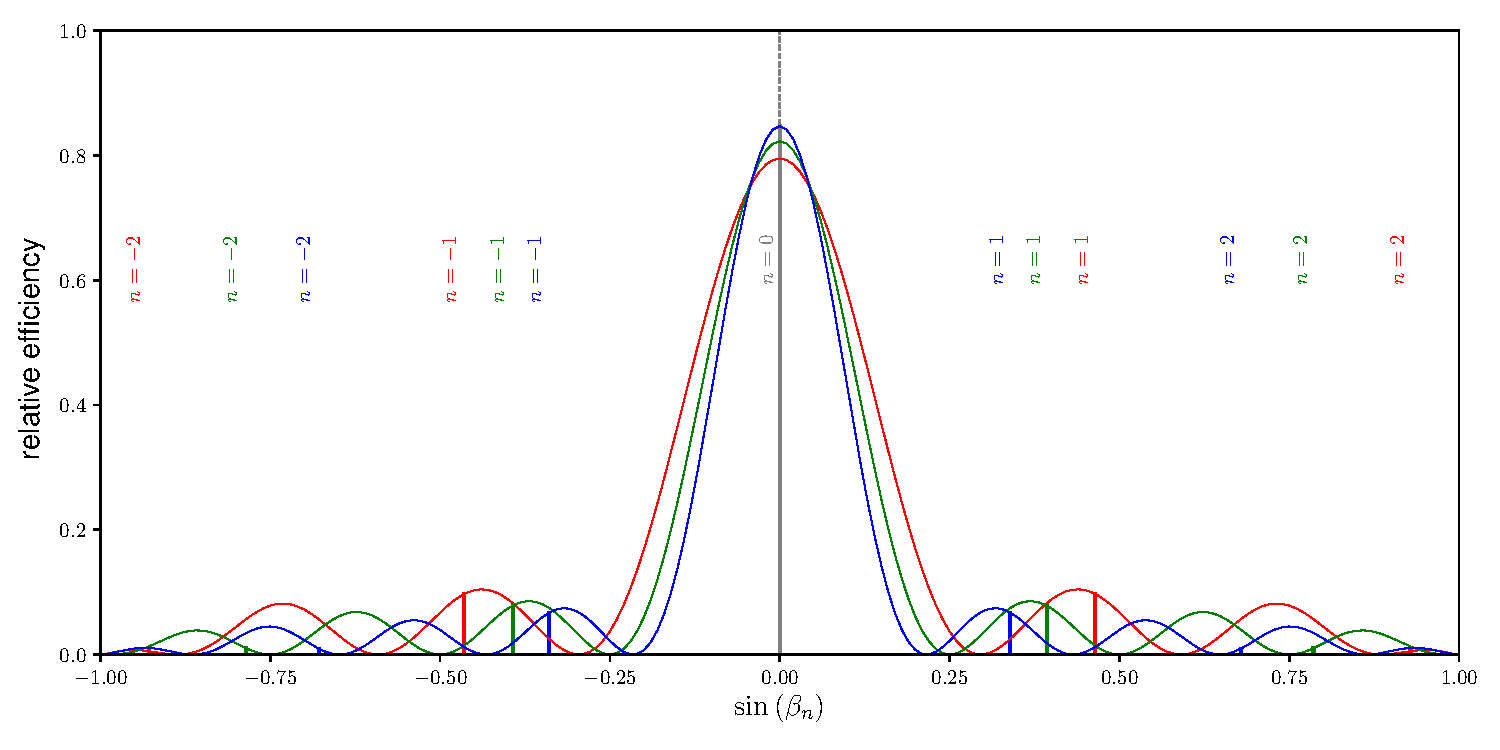
\includegraphics[scale=0.62]{Appendix-D/Figures/square_phase.pdf}
 \caption[Relative efficiency of a square-wave phase grating.]{Relative efficiency of a $\mathscr{W}/d = \SI{50}{\percent}$ square-wave phase grating at normal incidence with $h_0 / \lambda = 0.3$.}\label{fig:square_phase}
 \end{figure} 
This is illustrated in \cref{fig:square_phase} for a grating with $\mathscr{W} = d/2$, $\alpha = 0$ and $h_0 / \lambda = 0.3$, showing that the depth of the grating grooves, $h_0$, has an effect on the diffracted intensity in an analogous fashion to the aperture duty cycle, $\mathscr{W} / d$. 

\subsection{The Sinusoid}\label{sec:sinusoid_principle}
%%%%%%%%%%%%%%%%%%%%%%%%%%%%%%%%%%%%%%%%%--------------------------------------------------
As a next example, a sinusoidal amplitude grating is considered to have the following transmittance function: 
\begin{subequations}
\begin{equation}\label{eq:sin_amplitude_grating}
 G (x) = \mathcal{A} (x) = \frac{\mathcal{A}_0}{2} \left[ 1 + \sin (K x) \right] .
 \end{equation}
Because $\mathcal{A} (x)$ is constructed purely from $0^{\text{th}}$ and $\pm 1^{\text{st}}$ order spatial harmonics, only diffracted orders corresponding to Fourier coefficients with $n = 0, \pm 1$ should have a non-zero amplitude. 
This can be verified by inserting \cref{eq:sin_amplitude_grating} into \cref{eq:transmit_fourier_coeff} shows that $G_n = 0$ unless $n = 0, \pm 1$:
\begin{align}
\begin{split}
 G_n &= \frac{\mathcal{A}_0}{2 d} \int_{0}^{d} \left[ 1 + \sin (K x) \right] \mathrm{e}^{- i n K x} \dd{x} \quad \text{for } n = 0, \pm 1, \pm 2, \pm 3 \dotsc \\
 &= \frac{\mathcal{A}_0}{2 d} \int_{0}^{d} \left[ \mathrm{e}^{- i n K x} + \sin \left( K x \right) \cos \left( n K x \right) - i\sin \left( K x \right) \sin \left( n K x \right) \right] \dd{x} \\
 &= \frac{\mathcal{A}_0}{2 d} \left[ \underbrace{ \int_{0}^{d} \mathrm{e}^{- i n K x} \dd{x}}_\text{$d$ for $n=0$} + \overbrace{ \int_{0}^{d} \sin \left( K x \right) \cos \left( n K x \right) \dd{x} }^\text{always 0} - i \underbrace{ \int_{0}^{d} \sin \left( K x \right) \sin \left( n K x \right) \dd{x} }_\text{$\pm \frac{d}{2}$ for $n = \pm 1$} \right]
 \end{split}
 \end{align}
and therefore, the Fourier coefficients can be written as 
\begin{equation}\label{eq:sin_amplitude_grating_coef}
    G_n =
                \begin{cases}
                  -\frac{i \mathcal{A}_0}{4} , &\quad \text{for } n = 1 \\
                  \frac{\mathcal{A}_0}{2} , &\quad \text{for } n = 0  \\
                  \frac{i \mathcal{A}_0}{4} , &\quad \text{for } n = -1 \\
                  0 , &\quad \text{otherwise.}
                \end{cases}
 \end{equation}
This implies that the intensity of $0^{\text{th}}$ order should be four times the intensity of the $\pm 1^{\text{st}}$ orders while all other orders vanish: 
\begin{equation}\label{eq:sin_amplitude_grating_inten}
 \mathscr{E}_n \propto \frac{\cos \left( \beta_n \right)}{\cos \left( \alpha \right)} \norm{G_n}^2 \propto \frac{\cos \left( \beta_n \right)}{\cos \left( \alpha \right)}
                \begin{cases}
                  \frac{1}{16} , &\quad \text{for } n = \pm 1 \\
                  \frac{1}{4} , &\quad \text{for } n = 0  \\
                  0 , &\quad \text{otherwise}.
                \end{cases}
 \end{equation}
\end{subequations}
Although \cref{eq:sin_amplitude_grating} does not describe a physical grating in a general sense, this framework is useful to describe gratings with only one propagating order.  

A sinusoidal surface-relief grating with a groove-depth profile described by 
\begin{equation}
 h (x) = \frac{h_0}{2} \left[ 1 + \sin (K x) \right] ,
 \end{equation}
with $h_0$ as the maximum depth of the grating grooves, can be considered as a phase grating for a geometry where all portions of the groove are illuminated.  
In this case, a result different from \cref{eq:sin_amplitude_grating,eq:sin_amplitude_grating_coef,eq:sin_amplitude_grating_inten} is obtained with a phase function given by 
\begin{equation}
 \Phi (x) = \frac{\Phi_g}{2} \left[ 1 + \sin \left( K x \right) \right] = \Phi (x + d) ,
 \end{equation}
where $\Phi_g$ is the maximum phase shift that radiation picks up as it reflected from the groove structure [\emph{cf.\@} \cref{eq:laminar_phase}]. 
With amplitude assumed to be constant everywhere, the transmittance function is 
\begin{subequations}
\begin{equation}
 G (x) = \mathcal{A}_0 \mathrm{e}^{i \frac{\Phi_g}{2} \left[ 1 + \sin \left( K x \right) \right]}
 \end{equation} 
and then the following integral must be evaluated to determine the Fourier coefficients:
\begin{equation}\label{eq:sine_coef_integral}
 G_n = \frac{\mathcal{A}_0}{d} \mathrm{e}^{i \frac{\Phi_g}{2}} \int_{0}^{d} \mathrm{e}^{i \frac{\Phi_g}{2} \sin \left( K x \right)} \mathrm{e}^{- i n K x} \dd{x} \quad \text{for } n = 0, \pm 1, \pm 2, \pm 3 \dotsc .
 \end{equation}
\end{subequations}
The exponential sine term can be handled using a property of \emph{Bessel functions of the first kind}:
\begin{equation}\label{eq:Bessel_property}
 \mathrm{e}^{i \frac{\Phi_g}{2} \sin \left( K x \right)} = \sum_{m=-\infty}^{\infty} J_m \left( \frac{\Phi_g}{2} \right) \mathrm{e}^{i m K x} ,
 \end{equation}
where $J_m (\Phi_g / 2)$ is the $m^{\text{th}}$-order Bessel function. 
\begin{figure}
 \centering
 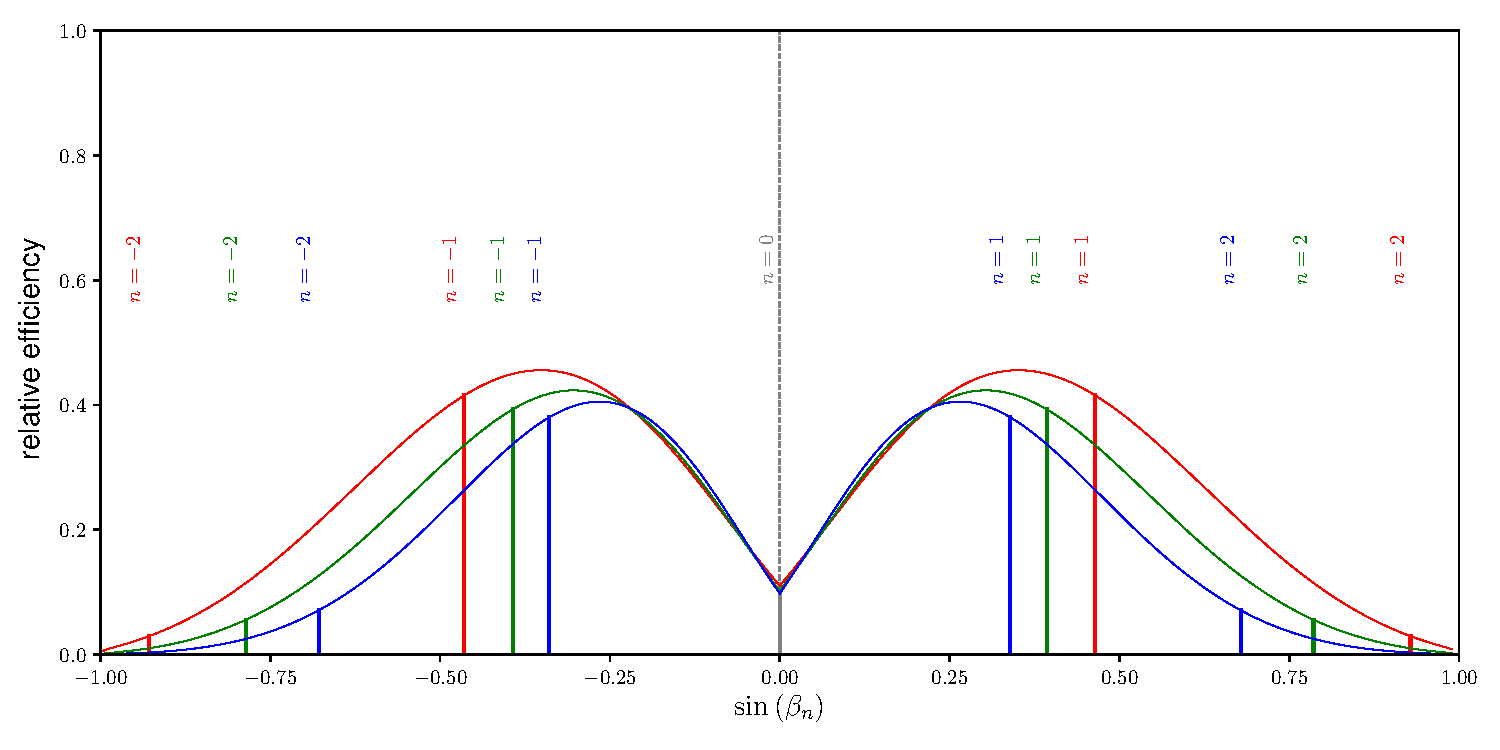
\includegraphics[scale=0.62]{Appendix-D/Figures/sine_phase.pdf}
 \caption[Relative efficiency of a sinusoidal phase grating.]{Relative efficiency of a sinusoidal phase grating at normal incidence with $h_0 / \lambda = 0.3$.}\label{fig:sine_phase} 
 \end{figure} 

Combining \cref{eq:sine_coef_integral,eq:Bessel_property} gives
\begin{align}\label{eq:G_terms_sine_phase}
 \begin{split}
 G_n &= \frac{\mathcal{A}_0}{d} \mathrm{e}^{i \frac{\Phi_g}{2}} \int_{0}^{d} \sum_{m=-\infty}^{\infty} J_m \left( \frac{\Phi_g}{2} \right) \mathrm{e}^{i \left( m - n \right) K x} \dd{x} \\
 &= \mathcal{A}_0 \mathrm{e}^{i \frac{\Phi_g}{2} } J_n \left( \frac{\Phi_g}{2} \right) \quad \text{for } n = 0, \pm 1, \pm 2, \pm 3 \dotsc ,
 %= \frac{\mathcal{A}_0}{d} \mathrm{e}^{i \chi} \int_{0}^{d} J_n \left( \chi \right) \dd{x} \\
 %= \mathcal{A}_0 \mathrm{e}^{i \chi} J_n \left( \chi \right)
 \end{split}
 \end{align}
which shows that orders of $\left| n \right| > 1$ can have a non-zero intensity depending on the value of $\Phi_g$, with the relative intensity of the $n^{\text{th}}$ order being 
\begin{equation}
 \mathscr{E}_n \propto \frac{\cos \left( \beta_n \right)}{\cos \left( \alpha \right)} \norm{G_n}^2 \quad \text{with} \quad \norm{G_n}^2 \propto \norm{J_n \left( \frac{\Phi_g}{2} \right)}^2. 
 \end{equation}
For a grating used at normal incidence, the diffraction efficiency becomes, using \cref{eq:laminar_phase} for $\Phi_g$, 
\begin{equation}
 \mathscr{E}_n \propto \frac{\cos \left( \beta_n \right)}{\cos \left( \alpha \right)} \norm{J_n \left( \pi \frac{h_0}{\lambda} \sqrt{1 - \left( \frac{n \lambda}{d} \right)^2 } \right)}^2  .
 \end{equation}
This is illustrated in \cref{fig:sine_phase} for $h_0 / \lambda = 0.3$, where it is seen that most diffracted efficiency is contained within orders $n = \pm 1$. 

\subsection{The Sawtooth}\label{sec:sawtooth_principle}
%%%%%%%%%%%%%%%%%%%%%%%%%%%%%%%%%%%%%%%%%--------------------------------------------------
The final grating groove shape to consider is the sawtooth, which is defined as a periodic function that increases with some slope over the duration of the period and then falls with infinite slope to start the cycle over again. 
If a hypothetical sawtooth amplitude grating is considered, the transmittance function is 
\begin{subequations}
\begin{equation}
 G (x) = \mathcal{A} (x) = \frac{\mathcal{A}_0}{d} x \quad \text{for } 0 < x \leq d ,
 \end{equation}
where $\mathcal{A}_0$ is the amplitude and $\mathcal{A}_0 / d$ is the slope of the sawtooth. 
Inserting this expression into \cref{eq:transmit_fourier_coeff} gives: 
\begin{equation}\label{eq:G_terms_square}
 G_n = \frac{\mathcal{A}_0}{d^2} \int_0^d x \mathrm{e}^{- i n K x} \dd{x} = \frac{\mathcal{A}_0 i}{2 \pi n} \quad \text{for } n = 0, \pm 1, \pm 2, \pm 3 \dotsc
 \end{equation}
so that $\mathscr{E}_n$ drops off as $n^{-2}$. 
\end{subequations}
Although this does not describe a physical diffraction grating, an ideal, blazed reflection grating can be treated as a surface where phase varies as a sawtooth: 
\begin{equation}
 \Phi (x) = \Phi_g \frac{x}{d} \quad \text{for } 0 < x \leq d , %\quad \text{and } \\
 %G \left( x \right) &= \mathcal{A}_0 \mathrm{e}^{i \Phi_g \frac{x}{d}} \quad \text{for } 0 < x \leq d ,
 \end{equation} 
where $\Phi_g$ is the phase shift difference between the top and bottom of a groove with depth $h_0$ [\emph{cf.\@} \cref{eq:laminar_phase}]. 
With Fourier coefficients for $G(x) = \mathcal{A}_0 \mathrm{e}^{i \Phi (x)}$ in this case given by 
\begin{align}
 \begin{split}
 G_n &= \frac{\mathcal{A}_0}{d} \int_0^d \mathrm{e}^{i \left( \frac{\Phi_g}{2 \pi} - n \right) K x} \dd{x} \\
 &= \frac{\mathcal{A}_0 i}{\left( \Phi_g - 2 \pi n \right)} \left( 1 - \mathrm{e}^{i \left( \Phi_g - 2 \pi n \right)} \right) \quad \text{for } n = 0, \pm 1, \pm 2, \pm 3 \dotsc ,
 \end{split}
 \end{align}
the scalar diffraction efficiency of the $n^{\text{th}}$ order is 
\begin{align}\label{eq:sawtooth_phase}
\begin{split}
 \mathscr{E}_n &\propto \frac{\cos \left( \beta_n \right)}{\cos \left( \alpha \right)} \norm{G_n}^2 \\
 \text{with} \quad \norm{G_n}^2  &\propto \frac{2 \left[ 1 - \cos \left( \Phi_g - 2 \pi n  \right) \right]}{\left( \Phi_g - 2 \pi n \right)^2} \propto \sinc^2 \left( \frac{\Phi_g}{2} - n \pi \right) . 
 \end{split}
 \end{align}

The sinc-squared function in \cref{eq:sawtooth_phase} indicates that the intensity of orders varies in a similar way to single-slit interference, where the maximum intensity corresponds to $\Phi_g = 2 \pi n$. 
However, in this case there exists a maximum for each diffracted order and $\Phi_g$ depends on the slope of the sawtooth with the groove depth given by $h_0 = d \tan \left( \delta \right)$:
%\begin{subequations}
\begin{equation}\label{eq:sawtooth_path}
 \Phi_g = \frac{2 \pi}{\lambda} d \tan \left( \delta \right) \left[ \cos (\alpha) + \cos (\beta_n) \right] .
 \end{equation}
Interference maxima then correspond to set of $n$ and $\lambda$ that satisfy the following relation:
\begin{equation}\label{eq:blaze_condition}
 n \pi = \frac{\Phi_g}{2} \implies \frac{n \lambda}{d} = \tan \left( \delta \right) \left[ \cos (\alpha) + \cos (\beta_n) \right] .
\end{equation}
Equating this with the generalized grating equation given by \cref{eq:off-plane_incidence_orders}, solving for $\tan \left( \delta \right)$ and recognizing the \emph{tangent of an average} trigonometric identity yields 
\begin{equation}
 \tan \left( \delta \right) = \frac{\sin (\alpha) + \sin (\beta_n)}{\cos (\alpha) + \cos (\beta_n)} \equiv \tan \left( \frac{\alpha + \beta_n}{2} \right),
 \end{equation}
%\end{subequations}
which shows that diffracted angles corresponding to maximum intensity are all given by $\beta_n = 2 \delta - \alpha$ and suggests that the slope of the sawtooth can be thought of as being similar to a mirror flat, where the reflected angle corresponds to the grating's blaze response. 
Inserting $\beta_n = 2 \delta - \alpha$ into \cref{eq:off-plane_incidence_orders} and then recovering the off-plane case using $\lambda \to \bar{\lambda} = \lambda \csc (\gamma)$ gives the equation for the \emph{blaze wavelength}: 
\begin{equation}\label{eq:blaze_wavelength_general}
 %\begin{split}
 \lambda_b = \frac{d \sin \left( \gamma \right)}{n} \left[ \sin \left( \alpha \right) + \sin \left( 2 \delta - \alpha \right)  \right] = \frac{2 d \sin \left( \gamma \right) \sin \left( \delta \right)}{n} \cos \left( \delta - \alpha \right)  ,
 %\end{split}
 \end{equation}
which describes a set of wavelengths and order numbers where diffraction efficiency is maximized. 
Using $\beta_n = 2 \delta - \alpha$ inserted into \cref{eq:sawtooth_path}, the phase shift corresponding to the blazed diffracted angle is
\begin{equation}\label{eq:sawtooth_path_blaze}
 \Phi_b  \equiv \frac{2 \pi}{\lambda} d \sin (\gamma) \left[ \sin (\alpha) + \sin (2 \delta - \alpha) \right] 
 \end{equation}
so that the diffraction efficiency is a special case of \cref{eq:sawtooth_phase} with $\Phi_g = \Phi_b$:
\begin{subequations}
\begin{align}\label{eq:sawtooth_phase_blaze1}
 \begin{split}
 \mathscr{E}_n &\propto \frac{\cos \left( 2 \delta - \alpha \right)}{\cos \left( \alpha \right)} \norm{G_n}^2 \\
 \text{with} \quad \norm{G_n}^2 &\propto \sinc^2 \left( \frac{d}{\lambda} \pi \tan \left( \delta \right) \sin (\gamma) \left[ \cos (\alpha) + \cos (2 \delta - \alpha) \right]  - n \pi \right) . 
 \end{split}
 \end{align}

For a scenario parameterized by fixed values of $\lambda$, $d$, $\delta$ and $\gamma$, the term $\norm{G_n}^2$ in \cref{eq:sawtooth_phase_blaze1} can be considered to behave as a function of $\alpha$, 
\begin{figure}
 \centering
 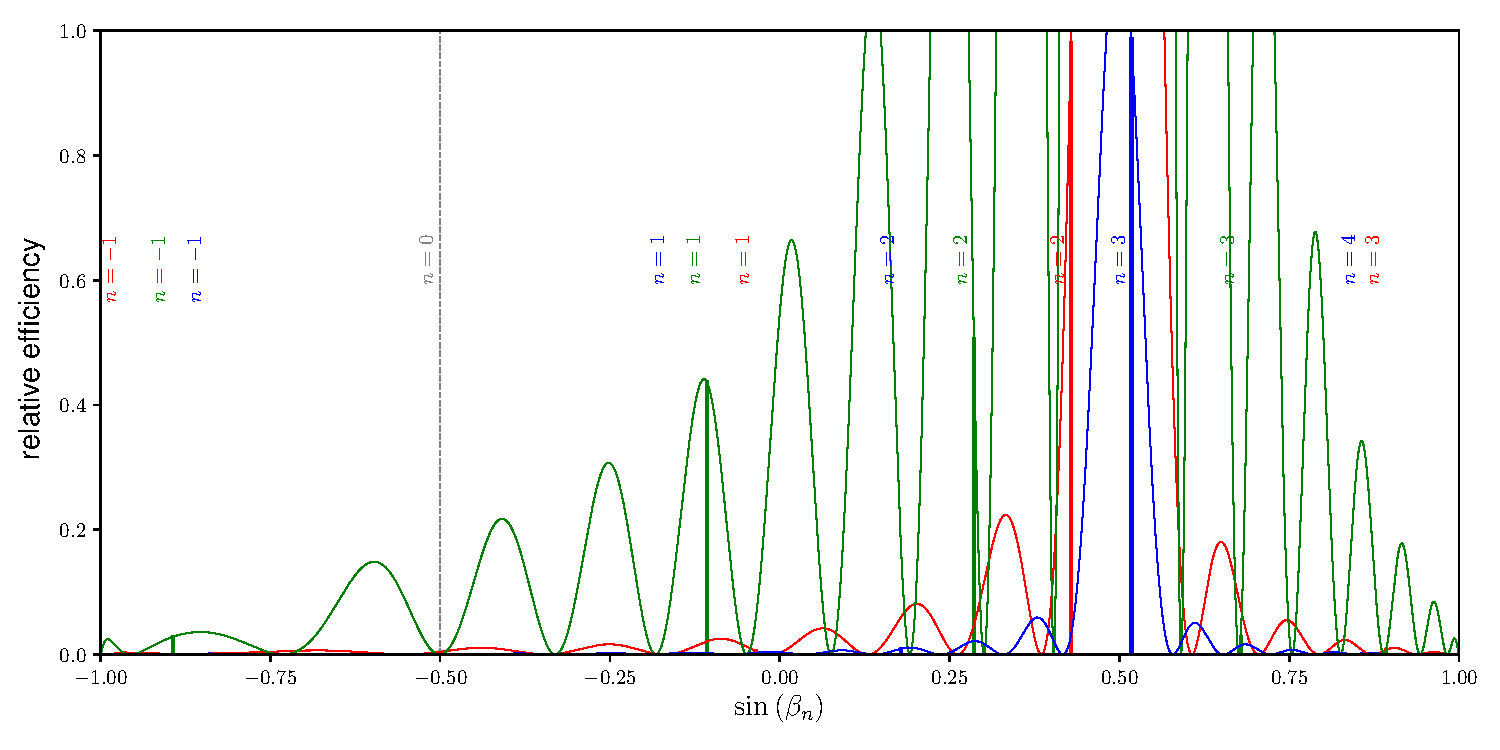
\includegraphics[scale=0.62]{Appendix-D/Figures/sawtooth_phase.pdf}
 \caption[Relative efficiency of a sawtooth phase grating.]{Relative efficiency of a sawtooth phase grating in a Littrow configuration with $\alpha = \delta = 30^{\circ}$.}\label{fig:sawtooth_phase} 
 \end{figure} 
which has local extrema characterized by values for $\alpha$ that satisfy the following partial derivative condition:
\begin{equation}\label{eq:blaze_partial1}
 \pdv{\alpha}(\norm{G_n}^2) \propto \pdv{f_n}{\Phi_b} \pdv{\Phi_b}{\alpha} = 0 \quad \text{with} \quad f_n \equiv \sinc^2 \left( \frac{\Phi_b}{2} - n \pi \right) .
 \end{equation}
Noting that 
\begin{equation}\label{eq:blaze_partial2}
 \pdv{f_n}{\Phi_b} = \pdv{f_n}{\Phi'} \underbrace{ \pdv{\Phi'}{\Phi_b}}_{1/2} = \frac{\sinc \left( \Phi' \right) \left[ \Phi' \cos \left( \Phi' \right) - \sin \left( \Phi' \right)  \right]}{\left( \Phi' \right)^2} \quad \text{with} \quad \Phi' \equiv \frac{\Phi_b}{2} - n \pi
 \end{equation}
and 
\begin{equation}\label{eq:blaze_partial3}
 \pdv{\Phi_b}{\alpha} = \frac{2 \pi}{\lambda} \sin (\gamma) \left[ \cos \left( \alpha \right) - \cos \left( 2 \delta - \alpha \right) \right] ,
 \end{equation}
the condition defined in \cref{eq:sawtooth_phase_blaze1} is guaranteed to be satisfied if $\pdv*{\Phi_b}{\alpha} = 0$ with $\alpha = \delta$ 
\end{subequations}
so that \cref{eq:blaze_wavelength_general} for the blaze wavelength reduces to 
\begin{equation}\label{eq:blaze_wavelength_Litt}
 \lambda_b = \frac{2 d \sin \left( \delta \right) \sin \left( \gamma \right)}{n} . 
 \end{equation}

An example of an efficiency response in a Littrow configuration with $\alpha = \delta = 30^{\circ}$ and $\sin \left( \gamma \right) = 1$ is plotted in \cref{fig:sawtooth_phase}. 
\begin{figure}
 \centering
 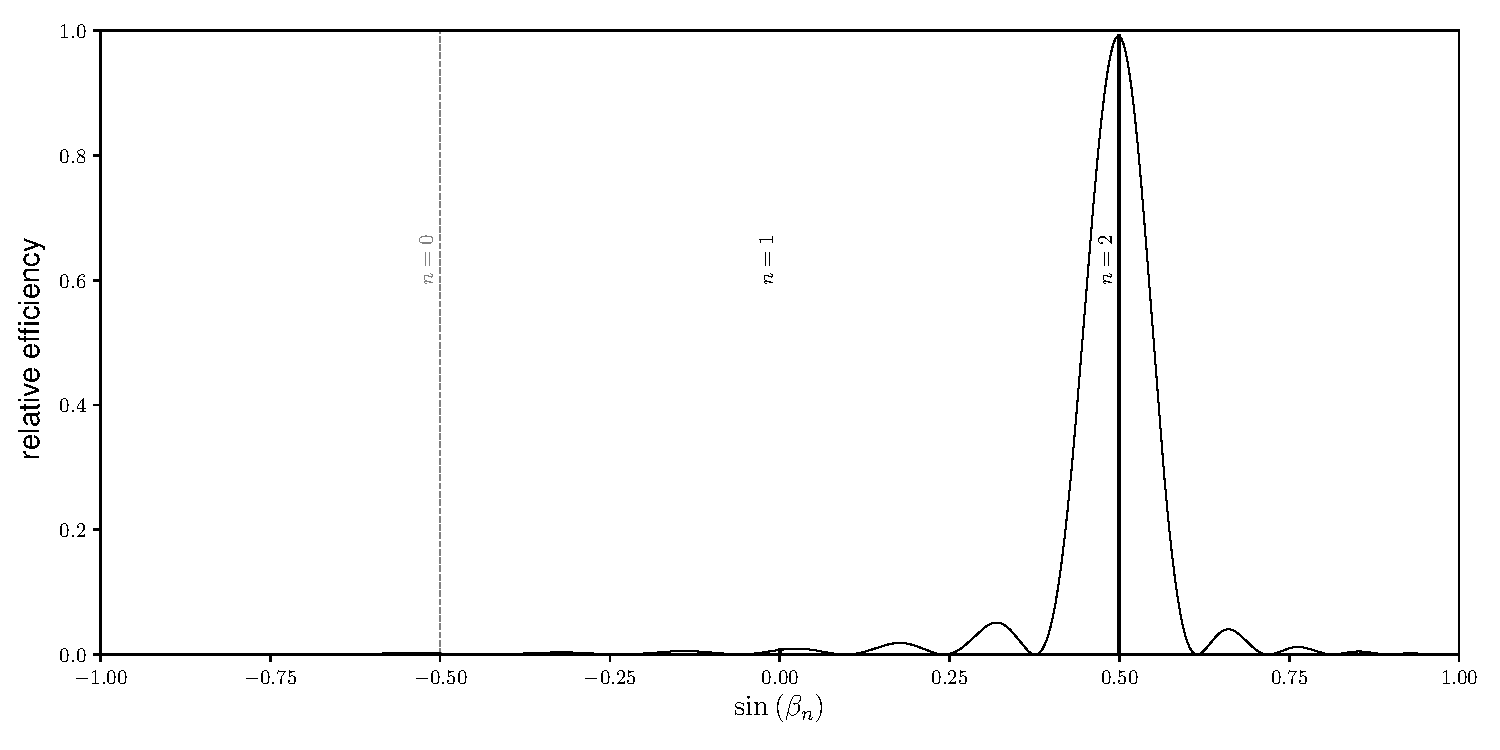
\includegraphics[scale=0.62]{Appendix-D/Figures/sawtooth_phase_blaze.pdf}
 \caption[Relative efficiency of a sawtooth phase grating at the blaze wavelength in second order.]{Relative efficiency of a sawtooth phase grating in a Littrow configuration with $\alpha = \delta = 30^{\circ}$, at the blaze wavelength for $n=2$.}\label{fig:sawtooth_phase_blaze} 
 \end{figure} 
Because $\lambda / d$ for red, green and blue do not satisfy exactly \cref{eq:blaze_wavelength_Litt} with $2 \sin \left( \delta \right) = 1$, diffraction efficiency is spread between orders rather than being concentrated at $\sin \left( \beta_n \right) = 0.5$. 
Red and blue values of $\lambda / d$, however, come close to satisfying the blaze condition for $n = 2$ and $n = 3$ and as a result, their diffraction efficiency is more concentrated near the blaze angle, as opposed to the case for green.  
A value of $\lambda / d = 0.5$, on the other hand, satisfies \cref{eq:blaze_wavelength_Litt} for $n=2$ and the blaze response of the grating is maximized, as illustrated in \cref{fig:sawtooth_phase_blaze}. 
Due to these properties, blazed gratings used in a Littrow configuration are optimal for maximizing $\mathscr{E}_n$ for a given $\beta_n$ and hence a given bandpass of interest [\emph{cf.\@} \cref{sec:grating_tech_dev}].

\section{Summary}\label{sec:appD_summary}
%%%%%%%%%%%%%%%%%%%%%%%%%%%%%%%%%%%%%%%%%-------------------------------------------------- 
Basic physics of diffraction gratings can be gleaned by considering Huygens-Fresnel principle applied to an array of periodically spaced slit sources, where grating behavior arises as the number of slits, $N$, becomes very large. 
According to the framework of Fraunhofer diffraction, the far-field diffraction pattern produced by a grating can be determined from the Fourier transform of its transmittance function, $G(x)$, which describes periodic variations in amplitude and phase caused by the grating. 
Reflection gratings can often be modeled as phase gratings determined by the path-length differences picked up as light reflects from a groove facet. 
While scalar this approach to modeling diffraction efficiency is limited due to its neglect of electromagnetic polarization and radiation interaction with materials, it is found that gratings with sawtooth-shaped groove facets have the ability to concentrate diffraction efficiency in the $n^{\text{th}}$ order over a particular spectral range. 
